% Options for packages loaded elsewhere
% Options for packages loaded elsewhere
\PassOptionsToPackage{unicode,pdfwindowui,pdfpagemode=FullScreen}{hyperref}
\PassOptionsToPackage{hyphens}{url}
\PassOptionsToPackage{dvipsnames,svgnames,x11names}{xcolor}
%
\documentclass[
  12pt,
  letterpaper,
]{article}
\usepackage{xcolor}
\usepackage[margin=1in]{geometry}
\usepackage{amsmath,amssymb}
\setcounter{secnumdepth}{-\maxdimen} % remove section numbering
\usepackage{iftex}
\ifPDFTeX
  \usepackage[T1]{fontenc}
  \usepackage[utf8]{inputenc}
  \usepackage{textcomp} % provide euro and other symbols
\else % if luatex or xetex
  \usepackage{unicode-math} % this also loads fontspec
  \defaultfontfeatures{Scale=MatchLowercase}
  \defaultfontfeatures[\rmfamily]{Ligatures=TeX,Scale=1}
\fi
\usepackage{lmodern}
\ifPDFTeX\else
  % xetex/luatex font selection
  \setmainfont[]{TeX Gyre Pagella}
  \setsansfont[]{TeX Gyre Pagella}
  \setmathfont[]{TeX Gyre Pagella Math}
\fi
% Use upquote if available, for straight quotes in verbatim environments
\IfFileExists{upquote.sty}{\usepackage{upquote}}{}
\IfFileExists{microtype.sty}{% use microtype if available
  \usepackage[]{microtype}
  \UseMicrotypeSet[protrusion]{basicmath} % disable protrusion for tt fonts
}{}
\usepackage{setspace}
\makeatletter
\@ifundefined{KOMAClassName}{% if non-KOMA class
  \IfFileExists{parskip.sty}{%
    \usepackage{parskip}
  }{% else
    \setlength{\parindent}{0pt}
    \setlength{\parskip}{6pt plus 2pt minus 1pt}}
}{% if KOMA class
  \KOMAoptions{parskip=half}}
\makeatother


\usepackage{longtable,booktabs,array}
\usepackage{calc} % for calculating minipage widths
% Correct order of tables after \paragraph or \subparagraph
\usepackage{etoolbox}
\makeatletter
\patchcmd\longtable{\par}{\if@noskipsec\mbox{}\fi\par}{}{}
\makeatother
% Allow footnotes in longtable head/foot
\IfFileExists{footnotehyper.sty}{\usepackage{footnotehyper}}{\usepackage{footnote}}
\makesavenoteenv{longtable}
\usepackage{graphicx}
\makeatletter
\newsavebox\pandoc@box
\newcommand*\pandocbounded[1]{% scales image to fit in text height/width
  \sbox\pandoc@box{#1}%
  \Gscale@div\@tempa{\textheight}{\dimexpr\ht\pandoc@box+\dp\pandoc@box\relax}%
  \Gscale@div\@tempb{\linewidth}{\wd\pandoc@box}%
  \ifdim\@tempb\p@<\@tempa\p@\let\@tempa\@tempb\fi% select the smaller of both
  \ifdim\@tempa\p@<\p@\scalebox{\@tempa}{\usebox\pandoc@box}%
  \else\usebox{\pandoc@box}%
  \fi%
}
% Set default figure placement to htbp
\def\fps@figure{htbp}
\makeatother


% definitions for citeproc citations
\NewDocumentCommand\citeproctext{}{}
\NewDocumentCommand\citeproc{mm}{%
  \begingroup\def\citeproctext{#2}\cite{#1}\endgroup}
\makeatletter
 % allow citations to break across lines
 \let\@cite@ofmt\@firstofone
 % avoid brackets around text for \cite:
 \def\@biblabel#1{}
 \def\@cite#1#2{{#1\if@tempswa , #2\fi}}
\makeatother
\newlength{\cslhangindent}
\setlength{\cslhangindent}{1.5em}
\newlength{\csllabelwidth}
\setlength{\csllabelwidth}{3em}
\newenvironment{CSLReferences}[2] % #1 hanging-indent, #2 entry-spacing
 {\begin{list}{}{%
  \setlength{\itemindent}{0pt}
  \setlength{\leftmargin}{0pt}
  \setlength{\parsep}{0pt}
  % turn on hanging indent if param 1 is 1
  \ifodd #1
   \setlength{\leftmargin}{\cslhangindent}
   \setlength{\itemindent}{-1\cslhangindent}
  \fi
  % set entry spacing
  \setlength{\itemsep}{#2\baselineskip}}}
 {\end{list}}
\usepackage{calc}
\newcommand{\CSLBlock}[1]{\hfill\break\parbox[t]{\linewidth}{\strut\ignorespaces#1\strut}}
\newcommand{\CSLLeftMargin}[1]{\parbox[t]{\csllabelwidth}{\strut#1\strut}}
\newcommand{\CSLRightInline}[1]{\parbox[t]{\linewidth - \csllabelwidth}{\strut#1\strut}}
\newcommand{\CSLIndent}[1]{\hspace{\cslhangindent}#1}



\setlength{\emergencystretch}{3em} % prevent overfull lines

\providecommand{\tightlist}{%
  \setlength{\itemsep}{0pt}\setlength{\parskip}{0pt}}



 


% -----------------------
% CUSTOM PREAMBLE STUFF
% -----------------------

% -----------------
% Title block stuff
% -----------------

% Abstract
\usepackage[runin]{abstract}
\renewcommand{\abstractnamefont}{\sffamily\small\bfseries}
\renewcommand{\abstracttextfont}{\sffamily\small}
\setlength{\absleftindent}{5pt}
\setlength{\absrightindent}{\absleftindent}

% Title
\usepackage{titling}
\pretitle{\par\begin{flushleft}\LARGE\sffamily\bfseries}
\posttitle{\par\end{flushleft}\vskip 10pt}

% Keywords
\newenvironment{keywords}
{\small\sffamily{\sffamily\small\bfseries{Keywords.}}}

% Authors
\usepackage{orcidlink}  % Create automatic ORCID icons/links
%\renewcommand{\and}{\end{tabular} \hskip 3em \begin{tabular}[t]{@{\hspace{0em}}l@{}}}
\preauthor{\begin{flushleft}
           \lineskip 1.5em}
\postauthor{\end{flushleft}}

% ------------------
% Section headings
% ------------------
\usepackage{titlesec}
\titleformat*{\section}{\Large\sffamily\bfseries\raggedright}
\titleformat*{\subsection}{\large\sffamily\bfseries\raggedright}
\titleformat*{\subsubsection}{\normalsize\sffamily\bfseries\raggedright}
\titleformat*{\paragraph}{\small\sffamily\bfseries\raggedright}

%\titlespacing{<command>}{<left>}{<before-sep>}{<after-sep>}
% Starred version removes indentation in following paragraph
\titlespacing*{\section}{0em}{2em}{0.1em}
\titlespacing*{\subsection}{0em}{1.25em}{0.1em}
\titlespacing*{\subsubsection}{0em}{0.75em}{0em}

% ------------------
% Headers/Footers
% ------------------
\usepackage{fancyhdr}
\pagestyle{fancy}
\fancyhf{}
\fancyhead[L,C,R]{}
\fancyfoot[L,C]{}
\fancyfoot[R]{\thepage}
\renewcommand{\headrulewidth}{1pt}
\fancypagestyle{plain}{%
    \renewcommand{\headrulewidth}{0pt}%
    \fancyhf{}%
    \fancyfoot[R]{\thepage}%
}
\renewcommand\footnoterule{\rule{\linewidth}{0.1pt}\vspace{5pt}}

% ------------------
% Captions
% ------------------
\usepackage[labelfont=bf,labelsep=period]{caption}
\captionsetup[figure]{font=footnotesize,justification=raggedright,singlelinecheck=false,format=hang}


% ---------------------------
% END CUSTOM PREAMBLE STUFF
% ---------------------------
\usepackage{float}
\usepackage{tabularray}
\usepackage[normalem]{ulem}
\usepackage{graphicx}
\usepackage{rotating}
\UseTblrLibrary{booktabs}
\UseTblrLibrary{siunitx}
\NewTableCommand{\tinytableDefineColor}[3]{\definecolor{#1}{#2}{#3}}
\newcommand{\tinytableTabularrayUnderline}[1]{\underline{#1}}
\newcommand{\tinytableTabularrayStrikeout}[1]{\sout{#1}}
\usepackage{dcolumn}
\usepackage{etoolbox}
\AtBeginEnvironment{longtblr}{\begin{singlespacing}}
\AtEndEnvironment{longtblr}{\end{singlespacing}}
\makeatletter
\@ifpackageloaded{caption}{}{\usepackage{caption}}
\AtBeginDocument{%
\ifdefined\contentsname
  \renewcommand*\contentsname{Table of contents}
\else
  \newcommand\contentsname{Table of contents}
\fi
\ifdefined\listfigurename
  \renewcommand*\listfigurename{List of Figures}
\else
  \newcommand\listfigurename{List of Figures}
\fi
\ifdefined\listtablename
  \renewcommand*\listtablename{List of Tables}
\else
  \newcommand\listtablename{List of Tables}
\fi
\ifdefined\figurename
  \renewcommand*\figurename{Figure}
\else
  \newcommand\figurename{Figure}
\fi
\ifdefined\tablename
  \renewcommand*\tablename{Table}
\else
  \newcommand\tablename{Table}
\fi
}
\@ifpackageloaded{float}{}{\usepackage{float}}
\floatstyle{ruled}
\@ifundefined{c@chapter}{\newfloat{codelisting}{h}{lop}}{\newfloat{codelisting}{h}{lop}[chapter]}
\floatname{codelisting}{Listing}
\newcommand*\listoflistings{\listof{codelisting}{List of Listings}}
\makeatother
\makeatletter
\makeatother
\makeatletter
\@ifpackageloaded{caption}{}{\usepackage{caption}}
\@ifpackageloaded{subcaption}{}{\usepackage{subcaption}}
\makeatother
\usepackage{bookmark}
\IfFileExists{xurl.sty}{\usepackage{xurl}}{} % add URL line breaks if available
\urlstyle{same}
\hypersetup{
  pdftitle={Inspiring Confidence and Easing Insecurity in the Pre-election period: The Effect of Recruiting Military Veterans on Confidence in 2024 US Elections},
  colorlinks=true,
  linkcolor={blue},
  filecolor={Maroon},
  citecolor={Blue},
  urlcolor={RoyalBlue},
  pdfcreator={LaTeX via pandoc}}



\title{Inspiring Confidence and Easing Insecurity in the Pre-election
period: The Effect of Recruiting Military Veterans on Confidence in 2024
US Elections}
% subtitles do not seem to work with article class?
%%\subtitle{}

\author{
{\bfseries \normalsize Isaiah Espinoza}%
 \\%
 \small University of Maryland, Department of Government and
Politics \\%
{\footnotesize \url{gespinoz@umd.edu}} \\\vspace{10pt}
}

\predate{}
\postdate{}
\date{}
\begin{document}

% for some reason this does not work in header
\renewcommand{\abstractname}{Abstract.}

% add the short title to the fancy header
\fancyhead[R]{Effect of Recruiting Military Veterans on Confidence in
2024 US Elections}
\fancyhead[L]{Isaiah}

\maketitle
%\noindent \rule{\linewidth}{.5pt}
\begin{abstract}
I report results from a recent survey experiment administered to test
whether publicized efforts to recruit veterans to work as election staff
and volunteers would improve public trust in elections and ease election
insecurity. Results of the survey experiment support the notion that
emphasizing veterans as the target of election worker recruitment
efforts eases pre-election insecurity. Expectations of electoral fraud
and concerns for voter safety were lower among those who read an
announcement that veterans are being recruited to work as election staff
and volunteers compared to those who read a control vignette where
veterans were not mentioned. Notable is that there was a significant
difference in confidence among those in the treatment condition who
believe that results of the 2020 election were illegitimate. In
addition, concerns over voter safety and potential for violence were
lower among those who received the treatment.
\end{abstract}
%\noindent \rule{\linewidth}{.5pt}


\setstretch{1.25}
\newpage{}

\subsection{Introduction}\label{introduction}

Election administration officials make efforts to sustain public trust
and confidence in the fairness and accuracy of elections, and attempt to
boost such confidence where it may be deprived. Concerns for safety have
developed among election staff and voters in more recent elections.
Regular measures are taken to enhance the \emph{trustworthiness} of the
electoral process through practices meant to improve the conduct,
transparency, or overall administration of elections in the United
States.

Although election officials undertake great efforts to enhance the
\emph{trustworthiness} of election administration, public
\emph{trust}\footnote{I adopt a distinction made between
  \emph{trustworthiness} and \emph{trust} in elections
  (\citeproc{ref-stewart2022}{Stewart 2022}). The ``\emph{worthiness}''
  of one's trust in the conduct and administration of elections is based
  on the extent that outcomes of an election reasonably follow the rules
  prescribed and can be adjudicated as such. The public's \emph{trust}
  in elections, however, is amendable to an indefinite number of factors
  that may be unrelated to the formal structure or procedures of
  election administration. I can recognize that my car is trustworthy
  prior to ever driving it because it is structurally sound; I have
  every reason to deem it \emph{worthy of my trust}. However, I don't
  trust my car because I am sure it is haunted.} in elections is a
psychological construct influenced by many things outside of election
official control such as partisanship or elite rhetoric
(\citeproc{ref-hooghe2018}{Hooghe 2018};
\citeproc{ref-sances2015}{Sances and Stewart 2015}). Moreover, a
person's evaluation of the election in hindsight is often influenced by
the election outcome itself (\citeproc{ref-daniller2019}{Daniller and
Mutz 2019}; \citeproc{ref-stewart2022}{Stewart 2022}). Thus, measures
taken by election officials can be undermined, trivialized, or made
irrelevant depending on how one feels after the election results have
come out.

Such volatile attitudes and evaluations post-election can leave a
lasting impression that election officials must contend with upon the
next election cycle (\citeproc{ref-bowler2024}{Bowler and Donovan 2024};
\citeproc{ref-levendusky2024}{M. Levendusky et al. 2024}). For instance,
we have witnessed many people's outright refusal to accept the 2020 U.S.
election results as legitimate despite consistent review of the evidence
confirming the results as fair and accurate. Such a case demonstrates
that public trust in elections is, at best, only partial to
trustworthiness of election administration in the United States.

One point of contention that election officials have faced in the past
regard evaluation of election workers. Previous literature has focused
on how voter interaction with election workers
(\citeproc{ref-claassen2008}{Claassen et al. 2008}), voting technology
(\citeproc{ref-herrnson2009}{Herrnson, Niemi, and Hanmer 2009}), and the
voter experience generally (\citeproc{ref-atkeson2007}{Atkeson and
Saunders 2007}), influences evaluations of election administration. As
such, election worker competency has been examined as a factor
significant to evaluations of performance of elections
(\citeproc{ref-hall2007}{T. Hall, Monson, and Patterson 2007};
\citeproc{ref-hall2009}{T. E. Hall, Quin Monson, and Patterson 2009}).
However, considering that individual perceptions and preconceived
notions play a huge role in cognition (\citeproc{ref-cikara2014}{Cikara
and Bavel 2014}; \citeproc{ref-vanbavel2021}{Van Bavel and Packer
2021}), it is reasonable to expect that the group an election worker
hails from would be an important influence upon the voter's evaluation
of the electoral process.

Supposing such is the case, we can expect that information about
\emph{who} (i.e., which groups) election officials are targeting in
publicized recruitment efforts would lessen particular election
insecurity, and concurrently, boost confidence. That is to say, it is
reasonable to expect that telling people \emph{who} will be working and
volunteering as election staff would ease election insecurity, and
therefore improve confidence that the election will be conducted fairly,
accurately, and safe for all involved.

I report results from a recent survey experiment administered to test
whether publicized efforts to recruit veterans to work as election staff
and volunteers would improve public trust in elections and ease election
insecurity. Results of the survey experiment show that emphasizing
veterans as the target of election worker recruitment efforts is
associated with greater confidence in elections and lower pre-election
insecurity. Expectations of electoral fraud and concerns for voter
safety were lower among those who read an announcement that veterans are
being recruited to work as election staff and volunteers compared to
those who read a control vignette where veterans were not
mentioned\footnote{The vignettes written were based on real news stories}.
Notable is that there was a significant difference in confidence among
those in the treatment condition who believe that results of the 2020
election were illegitimate. In addition, concerns over voter safety and
potential for violence were lower among those who received the
treatment.

This paper is structured as follows. First, I provide a brief background
on public trust in election administration. I synthesize a review of
relevant literature with a focus on how political and social science has
conceptualized and ascertained public trust in elections. Next, I supply
reasoning for why military veterans are singled out as the relevant
subset of the population expected to influence confidence in elections.
I provide testable hypotheses of the study before moving on to describe
the design of the survey, the measurement instruments therein, and the
conceptual and operational definitions of the variables of interest. I
explain my reasoning and method for constructing the primary dependent
variable, which I broadly refer to as \emph{confidence in elections}. I
close by offering my interpretation of the results and suggest potential
avenues for future inquiry.

\subsection{Background: Election Administration and Public
Confidence}\label{background-election-administration-and-public-confidence}

Election officials have tried hard to inspire confidence in the
administration and conduct of elections by improving the degree to which
elections are trustworthy. Development and implementation of procedures
such as post-election auditing of ballots and logic-and-accuracy testing
of ballot tabulation equipment are prominent examples adding to the long
history of efforts to enhance the trustworthiness of election
administration in the United States.

Prior to the year 2000, one of the main issues facing election
administration was recruiting enough election workers to volunteer at
the polls (i.e., poll workers) (\citeproc{ref-maidenberg1996}{Maidenberg
1996}). Election worker recruitment is still much of an issue in the
current era as it was then, perhaps worse
(\citeproc{ref-ferrer2024}{Ferrer, Thompson, and Orey 2024}). In
addition to ensuring election offices were adequately staffed, the
controversy of the 2000 general election made the public more attentive
to issues concerning the conduct and administration of elections. In
particular, voting technology (\citeproc{ref-herrnson2009}{Herrnson,
Niemi, and Hanmer 2009}) and election worker competence was of interest
in election studies (\citeproc{ref-claassen2008}{Claassen et al. 2008};
\citeproc{ref-hall2007}{T. Hall, Monson, and Patterson 2007};
\citeproc{ref-hall2009}{T. E. Hall, Quin Monson, and Patterson 2009}).
Following the passage of the Help America Vote Act in 2002, election
officials efforts to boost public confidence in the conduct and
administration of elections revolved primarily around the accuracy of
vote counts, ballot tabulation equipment or voting machines, the
commitment of election staff, and more
(\citeproc{ref-atkeson2007}{Atkeson and Saunders 2007}).

In 2024, election officials made valiant efforts to boost public
confidence elections within an intensified political climate that
appeared quite hostile to election officials
(\citeproc{ref-brennancenterforjustice2024}{Brennan Center for Justice
2024}; \citeproc{ref-edlin2024}{Edlin and Norden 2024}). Although
polling around the time indicated that most people thought that U.S.
elections would be run at least somewhat well
(\citeproc{ref-nadeem2024}{Nadeem 2024}), many election officials
nationwide took efforts to assuage the worry of those most skeptical.

Election anxiety was high in the lead up to the 2024 elections in the
United States. Concerns for voter safety and the prospect of political
violence remained prescient and compelled many local officials to
prepare for the worst (\citeproc{ref-doubek2024}{Doubek 2024};
\citeproc{ref-edlin2024}{Edlin and Norden 2024}). Election officials in
Washoe County, Nevada, installed panic buttons for election staff that
would alert a monitoring center to summon law enforcement
(\citeproc{ref-lincoln2024}{Lincoln 2024}). Nevada also passed a law
making it a felony to harass, threaten, or intimidate election workers
(\citeproc{ref-nevadasecretaryofstate2023}{Nevada Secretary of State
2023}). Leading up to election day, news outlets reported that election
work had become a seemingly dangerous job (\citeproc{ref-wire2024}{Wire
et al. 2024}). A Brennan Center survey report stated that,
``\ldots large numbers of election officials report having experienced
threats, abuse, or harassment for doing their jobs''
(\citeproc{ref-edlin2024}{Edlin and Norden 2024}). Concerns over the
fairness of elections and accuracy of vote counts intensified,
heightening concerns over the prospect of political violence and, in
turn, increased worry for the safety of voters and election workers
alike. Since election worker performance is significant to public
evaluation of elections, added safety concerns that drive out election
staff and repel volunteers can only detract from trustworthiness of the
institution.

\subsection{Literature Reivew}\label{literature-reivew}

Assessing the public's \emph{trust} in elections has not been
straightforward. Inquiry into public trust in elections has been
approached by scholars of political science in many different ways
(\citeproc{ref-cook2005}{Cook and Gronke 2005}), often distinguishable
by the scope of the research question and more or less constrained by
the particular conception of public trust. Quite often, trust in
election administration is conflated with trust in government writ
large, government legitimacy, government or system responsiveness, or
even satisfaction with democracy (\citeproc{ref-daniller2019}{Daniller
and Mutz 2019}). At this level, not only is the level of public trust in
elections sometimes vague, but there's little consideration over the
difference between such attitudes pre-election and post-election. In
contrast, a considerable amount of research tends to conceive of public
trust in accordance with the institution in question
(\citeproc{ref-atkeson2007}{Atkeson and Saunders 2007};
\citeproc{ref-hooghe2018}{Hooghe 2018}).

Election administration\footnote{It is important to point out here that
  election administration is just one institution that interacts with
  many other institutions and processes which form the electoral system
  \emph{writ large} (\citeproc{ref-stewart2022}{Stewart 2022}). The way
  in which I discuss the institution of election administration, as well
  as the way in which I discuss and distinguish public trust in
  elections from broader conceptions of public trust, is borrowed
  substantively from Stewart (\citeproc{ref-stewart2022}{2022})'s
  conceptual framework of the same. Distinctions between \emph{trust}
  and \emph{trustworthiness} and the notion of election administration
  as an institution are already apparent inspirations convenient for
  situating the theory of this research inquiry.} is just one part of
the larger set of institutions which form the electoral system. As such,
the performance of the institution along with the rest ``\ldots lends
credibility to the outcome of an election: whether it is considered by
citizens and the international community to be fair and legitimate.''
(\citeproc{ref-stewart2022}{Stewart 2022, 236}).

Trust in the conduct of elections concerns aspects of elections that
fall squarely within the institution of election administration. At this
level, for instance, public trust in elections is ascertained by
capturing assessments about the perceived accuracy of vote counts (e.g.,
whether votes are/were counted as intended).

Intuitively, enhancing public trust in elections would best be
accomplished by enhancing the \emph{trustworthiness} of the institution,
e.g., enhancing vote tabulation equipment and technology, conducting
audits. However, trust and confidence in elections has become ever more
precarious over the last few election cycles. Especially considering
public polling data since 2000 shows that confidence that votes were, or
would be, counted as intended was in a consistent decline despite
efforts towards bolstering election integrity and trustworthiness
(\citeproc{ref-sances2015}{Sances and Stewart 2015}). This is even more
pronounced considering the role that partisanship has had on such
confidence over accuracy of vote counts
(\citeproc{ref-sances2015}{Sances and Stewart 2015};
\citeproc{ref-stewart2022}{Stewart 2022}).

There's also stark difference in public trust before the election has
occurred compared to after, a phenomenon referred to as the
``winner-loser gap''; the ``winners'' are those who supported the
winning candidate and the ``losers'' are those who supported the losing
candidate. Much research has been dedicated to analyzing the sentiment
of electoral winners vs losers, and vice versa
(\citeproc{ref-daniller2019}{Daniller and Mutz 2019};
\citeproc{ref-nadeau1993}{Nadeau and Blais 1993}). Opinions of electoral
trust gathered after the election has occurred, however, are limited
considering the well-recognized impact that the electoral outcome itself
has on feelings of public trust in elections
(\citeproc{ref-daniller2019}{Daniller and Mutz 2019}).

As such, it is questionable whether we can characterize public trust in
the pre-election period as the same trust after the election results
have come out. The former is \emph{anticipatory}---i.e., the kind that
is more or less anxious given the uncertainties surrounding the
election. The latter is \emph{empirical}---a judgement discerned in
hindsight after the experience of the election event has occurred. As
discussed by Stewart (\citeproc{ref-stewart2022}{2022}), not only was
confidence in vote count accuracy influenced by the voter experience,
but so too were evaluations of election officials
(\citeproc{ref-stewart2022}{2022, 242--43}). Not to mention the
influence that the election results would also have on such evaluations.
In other words, evaluations of trust considered in hindsight are
influenced by the voter experience and the outcome of the election
results. This study, in contrast, focuses primarily on that
\emph{anticipatory} kind of confidence, which speaks more to those
insecurities based on perceptions of the institution's trustworthiness
than upon the particular voter experience.

Regardless of the measures taken by election officials to boost public
confidence in the \emph{trustworthiness} of election administration
(e.g., conducting audits, testing election machines), public
\emph{trust} and confidence in elections more generally is apt to shift
dramatically post-election based on factors such as partisanship, elite
rhetoric, particular state policies, and more
(\citeproc{ref-carter2024}{Carter et al. 2024};
\citeproc{ref-coll2024a}{Coll and Clark 2024};
\citeproc{ref-nadeau1993}{Nadeau and Blais 1993}). Moreover, prior
research has found that evaluation of election workers themselves are an
important factor when it comes to levels of public confidence in the
electoral process (\citeproc{ref-claassen2008}{Claassen et al. 2008};
\citeproc{ref-hall2007}{T. Hall, Monson, and Patterson 2007};
\citeproc{ref-hall2009}{T. E. Hall, Quin Monson, and Patterson 2009}).
Such studies focused on the quality of the voter experience with
reference to the interaction between voter and election worker.

Beyond the general competence of election workers, however, the quality
of the voter experience may be influenced merely by prior impressions
about \emph{who} comprises election staff and volunteers. Political and
other social science researchers have recognized for some time the power
that group identity can have over attitudes and perception
(\citeproc{ref-vanbavel2021}{Van Bavel and Packer 2021};
\citeproc{ref-xiao2016}{Xiao, Coppin, and Van Bavel 2016};
\citeproc{ref-xiao2012}{Xiao and Van Bavel 2012}). As such, we can
expect that information identifying the particular groups being
recruited to serve as election staff will be enough to improve
confidence in elections, and lessen expectations of electoral fraud. The
next section elaborates on the proposed theory, terms utilized, and why
military veterans are of particular interest in this regard.

\section{Theory}\label{theory}

This theory is constrained to public confidence in the administration of
elections in the United States. To be clear, the scope conditions in
which this theory applies concern public trust and distrust in election
administration in the anticipatory period prior to the election event.
Moreover, this study is, to a limited extent, indirectly related to
public regard about veteran members of the U.S. Armed Forces.

\subsection{Trust and Distrust in
Elections}\label{trust-and-distrust-in-elections}

The theoretical relationship between trust and distrust is important to
understand, especially when it comes to the dependent outcome of
interest. Before going further, it is necessary to explicate the
conception \emph{confidence in elections} with respect to trust and
distrust.

Trust is, after all, merely \emph{belief} held in the face of
uncertainty. Trust is reliance on the veracity of belief in the face of
uncertainty. Said another way, trust is assured belief dependent on its
supposed veracity; a state of certainty with respect to some belief or
judgement. It is ``assured'' because it is one's belief that relies on
something rather than nothing. Hence quantitative methods of the
sciences are replete with things such as \emph{confidence} intervals
around our estimates. Therefore, I understand trust to refer to the
state or quality of certainty around one's beliefs or expectations; the
extent to which one is assured of their expectations regarding what is
or what will be the case.

The kind of \emph{trust in elections} I refer to concerns the
expectations drawn up from one's judgement about the functioning of the
electoral process---the extent to which one is assured in the belief
that the electoral process will be fairly and accurately administered. I
follow the notion of public trust in elections explicated by Stewart
(\citeproc{ref-stewart2022}{2022}),

\begin{quote}
``Public trust in U.S. election institutions comes down to whether
voting machines accurately record votes, voter registration systems
accurately record those eligible to vote, geographic information systems
accurately assign voters to voting districts, election-night reporting
systems accurately aggregate and communicate election results to
officials and the public, and postelection audit and canvassing
procedures proceed impartially and in accordance with the law.''
(\citeproc{ref-stewart2022}{2022, 236})
\end{quote}

That being said, I also account for expectations of electoral fraud,
which I refer to as \emph{distrust} in elections distinguished from
trust. Distrust in this sense is also a belief, an expectation, about
the anticipated functioning of the process. Note, however, that the
prefix \emph{dis-} in distrust implies ``apart'', ``lack of, not'' or
``opposite''. Conventionally, distrust is defined simply as the absence
of trust, thus denoting a simple inverse and mutually exclusive
relationship. However, as it concerns the psychology of an individual,
\emph{a lack of trust doesn't necessarily imply opposite expectations or
opposing beliefs}. In particular, a lack of trust that votes will be
accurately recorded, etc., doesn't necessarily imply inversely
proportional expectations that electoral fraud will occur. In other
words, although the relationship between trust and distrust is inverse,
this relationship is not mutually exclusive.

A person who is certain that electoral fraud will occur clearly lacks
trust in elections; an expectation that electoral fraud will occur
necessarily implies a lack of trust in elections regardless of positive
expressions of trust. However, the reverse isn't also true; expressing a
lack of trust in elections \emph{doesn't necessarily imply} an
expectation that electoral fraud will occur. Rather, a lack of trust
implies an absence of assurance in the belief that the process will be
conducted fairly and accurately---a lacking quality of certainty around
said belief. An absence of such assurance denotes a state of
\emph{insecurity}. Other sources of uncertainty may challenge a person's
confidence regarding the integrity of elections independent from
anything that would lead them to believe electoral fraud will occur or
has occurred. However my use of distrust refers to the assured belief
that the outcome will be invalid---that outcomes will be independent of
the process as prescribed, thus rendering outcomes as arbitrary.
Specifically, distrust implies assurance in the belief that electoral
fraud will occur.

As such, trust and distrust represent opposing degrees of confidence
along the same spectrum. However, despite the inherent contrast, one can
hold both positive degrees of trust and distrust, feeling relatively
confident in both respects. Accordingly, \emph{equivalent degrees of
trust and distrust cancel out}, rendering one relatively more insecure
about their expectations of the future despite the fact that they may
report feeling confident in either direction respectively. When trust
and distrust are considered reflective of one's confidence about future
expectations, then both can be placed along the same spectrum.
Therefore, a lack of confidence denotes insecurity.

This means that a person's baseline level of confidence in elections
must take into account their present degree of distrust---i.e., their
expectations of electoral fraud. Something may cause a person to have
greater expectations that election fraud will occur, which in turn will
always lower their trust in elections. In contrast, a person's trust in
the integrity of the electoral process is reduced by the extent to which
they expect that electoral fraud will occur.

Thus, it follows that a person distrusts the integrity of the electoral
process to the extent that they are to some extent certain that
electoral fraud will occur or has occurred. They are, perhaps, poised to
discount election results as invalid or illegitimate in advance. Either
way, both trust and distrust refer to some positive degree of confidence
(i.e., assurance) regarding one's expectations. They are distinguished
by reference to either the normative idea about what \emph{should} come
about, or what is \emph{supposed} to come about given the logical
structure and integrity of the process. If the structure and integrity
of some process is coherent and secure, respectively, then the outcome
that follows will be valid. Should the integrity of that process be
damaged or opaque, then the process becomes vulnerable and validity of
the results are open to challenge. With respect to the administration of
U.S. elections, the confident voter expects that votes will be counted
as voters intend, election staff will competently administer elections,
election technology will be secure from nefarious tampering, and that
the process will be fair for all involved.

\subsection{Why Veterans}\label{why-veterans}

Election officials don't focus on recruiting people of a particular
demographic, status, class, or prestige in order to shore up public
trust in elections, and they don't discriminate recruitment efforts
based on who the public thinks is best suited to secure elections from
fraud.

Election officials are likely to be agnostic as to who dedicates their
time to civil service such as election work. Especially since staffing
has been an issue since at least the 1990s
(\citeproc{ref-ferrer2024}{Ferrer, Thompson, and Orey 2024};
\citeproc{ref-maidenberg1996}{Maidenberg 1996}). In 2020, such efforts
were made far more difficult by the COVID-19 pandemic
(\citeproc{ref-abbate2020a}{Abbate 2020}; \citeproc{ref-mena2020}{Mena
2020}). There's no special reason to target veterans for recruitment
above other groups. Indeed, there's no reason to discriminate
recruitment efforts at all if the point is purely to fill staffing
vacancies.

Veteran military service members are, after all, civilians; Civilians
with shared (but varied) experience and status of prior military
service, but who are no more or less qualified for this civil
service\footnote{Research is limited and mixed on whether veterans in
  general are more inclined, however (\citeproc{ref-nesbit2011}{Nesbit
  and Reingold 2011}).} than non-veteran civilians. To be frank,
announcements about concerted efforts to recruit veterans as election
workers should not reasonably influence one's trust that votes will be
counted more accurately, or that election fraud will not occur; there is
no known evidence demonstrating that actually employing veterans as
election staff or volunteers further improves the safety, security, and
overall integrity of elections in the United States. Moreover, there's
no known evidence of positive influence on public perceptions of said
outcomes when voters encounter military veterans working as staff or
volunteers at elections sites.

Rather, the claim that recruiting veterans to work as election staff and
volunteers would improve public confidence in elections emerges as
non-profit organizations---mainly comprised of veteran and military
family members themselves---operate under, and promote, that assumption
(\citeproc{ref-lawrence2024}{Lawrence 2024};
\citeproc{ref-looker2024}{Looker 2024};
\citeproc{ref-wentling2024}{Wentling 2024}). Non-profit groups of late
have made incredible strides in targeted recruitment efforts under the
notion that veterans are uniquely capable, committed, and best fit to
serve the needs of the United States as civil servants and volunteers at
election sites. Indeed, this study can be seen as a test of a particular
assumption that veterans have about themselves---the assumption that
their mere presence and civic engagement will inspire confidence in
elections among the public.

There was a sudden push to target veterans for recruitment efforts that
arose shortly after the events on Capitol Hill on January 6th, 2021.
After the 2020 election, large efforts were made to recruit military
veterans and their families to work or volunteer as election staff
(\citeproc{ref-nflfootballoperations2022}{NFL Football Operations 2022};
\citeproc{ref-wetheveterans2022}{We The Veterans 2022}). Prior to that
point, young people were sometimes given special mention as targets of
election worker recruitment efforts (\citeproc{ref-herndon2020}{Herndon
2020}; \citeproc{ref-powerthepolls2020}{Power the Polls 2020}).
Generally, however, recruitment efforts cast a wide net, indiscriminate
of who applies (\citeproc{ref-conde2020}{Conde 2020};
\citeproc{ref-ross2020}{Ross 2020}).

One can speculate that the motivation to associate military veterans
with civic engagement and democracy may be intended to counter negative
perceptions and impressions given by the proportion of veteran service
members arrested for taking part in the events on January 6th
(\citeproc{ref-jensen2022a}{Jensen, Yates, and Kane 2022};
\citeproc{ref-loewenson2023}{Loewenson 2023};
\citeproc{ref-milton2021}{Milton and Mines 2021}). Especially with
regard to research demonstrating that willingness to support violent
efforts to overturn election results (in support of Trump) is, on
average, more common among veterans than among matched samples of
non-veterans (\citeproc{ref-pape2024}{Pape et al. 2024}). This is in
addition to a strengthened association portrayed in media outlets
between military veterans and militias
(\citeproc{ref-steinhauer2020}{Steinhauer 2020}). Prior research has
substantiated such a connection between veterans and militia groups.
Cooter (\citeproc{ref-cooter2024}{2024}) notes from her 3-year
ethnographic fieldwork among Michigan militia members that,
``\ldots approximately 40\% of militia leaders and 30\% of members had
previous military experience. Most of these veterans actively sought out
such groups, as opposed to being recruited by them'' (see also
\citeproc{ref-cooter2013}{Cooter 2013}). Thus, countering such
associations by promoting a different image of veterans to the mass
public and veterans alike seems like a reasonable motivation. Yet such
speculation is just that.

The key findings of literature on confidence in elections hardly point
to public regard for veterans as a mechanism for the theoretical
expectations of improving overall confidence in elections and improving
feelings of voter safety at election sites. Comparable research finds
that confidence in elections is increased through elite rhetoric from
fellow partisans affirming legitimacy of elections
(\citeproc{ref-clayton2023}{Clayton and Willer 2023}), or through the
provision of information about the electoral process or other official
messaging of election officials themselves
(\citeproc{ref-gaudette2025}{Gaudette et al. 2025}). Neither of the
studies just cited, however, consider attitudes or sentiment about
veterans as a source for dispelling distrust and improving trust in
elections. To be clear, there is no immediate ``puzzle'' in the
literature that immediately draws out public sentiment for military
veterans as a source for bolstering confidence in elections. That being
said, the general public perception, attitudes, or even stereotypes
about military veterans are significant to consider.

It is important to make clear two considerations that underpin the
notion that information about veterans will improve trust and quell
distrust in elections. First, positive public regard for veterans
\emph{in general} is sufficient to elicit greater trust and lower
distrust in elections despite the fact that information about veterans
as election workers, or even merely information on efforts to recruit
veterans, has no bearing on the actual integrity of the electoral
process. An underlying assumption here is that there \emph{is} something
special about veterans, but this doesn't include a proposition on
exactly \emph{what} that special something might be in theory. This is
partly due to the limited research available on public regard for
veterans, specifically in terms of elucidating an underlying mechanism
for such positive favor. Moreover, there is limited research on public
opinion about former and active military service members distinguished
separately from public opinion about the military as an institution in
general. Endorsement or support of government policies intended to
benefit veterans specifically (e.g., federal funding on veteran
healthcare) are easy to conflate as interchangeable with public
attitudes about veterans as a group in particular. This, in turn,
permits general expectations of positive influence due to the public's
overarching positive regard for veterans, but disallows for expectations
regarding how respondents would actually process and interpret a
treatment that only mentions efforts to recruit them for election work.
In short, we are sure that people sustain positive views for veterans
generally, but beyond that I make no special effort to propose and
examine why that is the case in greater detail.

The evidence that can be gathered concerning public regard for military
veterans shows that, generally, veterans are perceived favorably among
the general public; although military recruitment shows a downward trend
as of late, public perceptions of veterans are overwhelmingly positive
(\citeproc{ref-kleykamp2023}{Kleykamp, Schwam, and Wenig 2023}). In my
review of the literature, I found only one study which assessed public
opinion about veterans specifically and examined whether attitudes
differed by group (\citeproc{ref-kleykamp2018}{Kleykamp, Hipes, and
MacLean 2018}). Kleykamp, Hipes, and MacLean
(\citeproc{ref-kleykamp2018}{2018}) investigated the extent to which
positive regard for military veterans in terms of both social distance
and deservingness varies across different groups, and the extent to
which such support is exaggerated. Their research found that levels of
support for veterans tended to be predictably lowest, but also most
exaggerated, among those who were younger and non-White. Determining
what groups hold special favor for veterans still leaves it unclear as
to what it is about veterans that engenders greater confidence in
elections. Yet, generally, all groups expressed exaggerated support for
veterans in more than one way (\citeproc{ref-kleykamp2018}{Kleykamp,
Hipes, and MacLean 2018}), suggesting that public regard for veterans is
prescribed by widespread social norm.

This is taken together with literature suggesting that public trust in
elections is malleable to factors, experiences, events, or phenomena
that range in logical relevance to the actual structure or
administration of elections. On the one hand, public trust is, indeed,
influenced by information specifically about the processes of conducting
elections (\citeproc{ref-gaudette2025}{Gaudette et al. 2025}). On the
other hand, the public's trust in elections is not beholden to the
demonstrated \emph{trustworthiness} of the institution of election
administration. Thus the first consideration is simply that the positive
public regard for veterans in general may function sufficiently as a cue
to elicit greater trust in elections despite relevance.

Second, veterans are a particularly potent group where mention of one's
veteran status seems to have a positive, calming, or nullifying effect
on attitudes. More so than just the general positive favor afforded to
veterans, the group appears to have a somewhat pacifying effect on
negative or otherwise contemptible discrimination, prejudice, and social
stigma. For instance, recent research shows that, during his campaign in
the 2020 Democratic Primaries, Pete Buttigieg's military background
mitigated discrimination against him when he was presented as a veteran
married to a man (\citeproc{ref-magni2024}{Magni and Reynolds 2024}).
Similar research has also found that a candidate's veteran status
affords them better evaluations regarding competency in particular issue
areas (e.g., war competence) (\citeproc{ref-hardy2019}{Hardy et al.
2019}; \citeproc{ref-teigen2013}{Teigen 2013}). Moreover, veteran status
seems to mitigate or nullify usual stigmas associated with mental
illness. That is to say, there is negative stigma associated with mental
illness (\citeproc{ref-corrigan2002}{Corrigan et al. 2002}) and such
stigma incurs labor market discrimination
(\citeproc{ref-hipes2016}{Hipes et al. 2016}), but evidence suggests
that veteran status overrides such stigma and discrimination
(\citeproc{ref-maclean2014}{MacLean and Kleykamp 2014}). Or, in another
light, mental illness is seemingly more \emph{understandable} (i.e.,
permissible) for veterans given the presumptive reasons for their mental
strife. And media framing as such plays an important role on public
perception (\citeproc{ref-kleykamp2015}{Kleykamp and Hipes 2015}).
Relatedly, attitudes about homelessness and PTSD---ranging from
perceived causes of homelessness, whether the federal government should
dedicate more resources, perceived effectiveness of policies, to
compassion for homeless individuals---are generally more favorable for
the homeless population among veterans than for the homeless population
of general adults (\citeproc{ref-tsai2021}{Tsai et al. 2021}). Such
effects primarily pertain to attitudes about individual people or groups
(e.g., a political candidate, prospective employees, the homeless
population). The capacity of one's veteran status to pacify prejudice,
discrimination, and stigma likely extends out to quell negative and
disfavorable attitudes regarding institutions to a similar extent, e.g.,
distrust.

The question emerged in light of the recent surge of efforts nationwide
to recruit veterans to serve as election workers
(\citeproc{ref-lawrence2022}{Lawrence 2022};
\citeproc{ref-wentling2024}{Wentling 2024}) midst an environment where
election insecurities were heightened and intensified. Bearing that in
mind, the heightened insecurities in anticipation of upcoming elections
do not merely pertain to the election outcome (e.g., who wins), but to
one's general sense of confidence in the integrity of elections
administration and to the safety of casting a ballot in-person.

Given the heightened tensions and electoral anxieties, the expectations
surrounding the unique pacifying effect that veterans have on attitudes
about individuals or other groups is extended to determine whether a
similar effect is found when the target of one's consideration is not
just a person or group but the institution of election administration
itself. Thus the second consideration for ``why veterans'' are expected
to dispel distrust in elections pertains to pacifying effect of negative
or disfavorable attitudes observed in relevant literature.

The stimulating influence of veterans as a group in the abstract is
expected to counteract distrust and insecurity pertaining to the
institution of elections administration, as well as inspire greater
confidence in the same. There's scant research or evidence available to
postulate a well-formed theory on the mechanism underlying the expected
effects of veterans as a group on attitudes about institutions and
processes, rather than on attitudes about persons or groups. What may be
posited at best, however, is that distrust and insecurity in elections
among the public is expectedly reduced to some extent through generally
positive public regard for military veterans and their unique capacity
to quell disfavorable attitudes.

\subsection{Hypotheses}\label{hypotheses}

The outcome of interest is \emph{confidence in elections}, which refers
to trust in elections---i.e., expectations that elections will be
administered fairly and accurately---compensated by distrust in
elections---i.e., expectations that electoral fraud will occur.
Considering the generally positive perception afforded to veterans by
the public, it is reasonable to suspect that efforts that promote
recruitment of veteran military service members to work as election
staff and volunteers would boost public \emph{confidence in elections
administration}. Indeed, that is the primary hypothesis of this study.
Although citizens may vote in various ways across the country (e.g., by
mail, ballot drop box, in-person), the simple announcement that election
officials are engaging in efforts to recruit veterans to work as
election staff may boost confidence in elections administration
regardless of how, or whether, an individual plans to vote. Formally,

\begin{quote}
H\textsubscript{1}: Announcements that election officials are recruiting
miilitary service veterans to work as election staff and volunteers will
be associated with greater confidence in elections administration
compared to announcements that do not mention military veterans.
\end{quote}

Asking participants whether they supported programs intent on recruiting
anyone to work as election staff would garner support regardless of the
target group. Considering that support and admiration for veterans is
generally high among the population
(\citeproc{ref-kleykamp2023}{Kleykamp, Schwam, and Wenig 2023}), then
discerning the impact on one's confidence would require a survey
experiment designed to determine whether publicized recruitment efforts
targeting veterans as a group would have any special effect on
confidence in elections administration.

In addition, prior research has shown that confidence that one's own
vote would be counted as intended has been much stronger than confidence
that votes nationwide would be treated likewise
(\citeproc{ref-sances2015}{Sances and Stewart 2015};
\citeproc{ref-stewart2022}{Stewart 2022}). In other words, the public is
more trusting of elections closer to home. Taking into account that
confidence is lower for elections conducted outside of one's local area,
then information that veterans are being recruited to help conduct
elections in locations beyond one's locale may close this gap between
confidence in elections within one's local area and confidence in
elections elsewhere. Although it may be difficult to discern whether
recruiting veteran service members would improve confidence in elections
near one's local area in light of such hometown favoritism, a positive
effect on confidence in elections held beyond one's local area---where
confidence is already expectedly lower---can help discern the impact of
the group alone on public opinion. Therefore, any observed disparity of
confidence in elections between those within one's local area and those
beyond will be smaller among those who are presented with information
about election official recruitment efforts of veteran service members.
Formally,

\begin{quote}
H\textsubscript{2}: Differences in confidence in elections in one's
local area and confidence in elections in Maricopa County, AZ, will be
smaller among those who are presented with an announcement that election
officials are recruiting miilitary service veterans to work as election
staff and volunteers compared to those presented with an announcement of
recruitment efforts that do not mention military veterans.
\end{quote}

Since the results and events following the 2020 election loomed large in
anticipation of the U.S. 2024 general elections, it is reasonable to
take into account beliefs about legitimacy of the 2020 election. This
group who denies the legitimacy of the 2020 election results were
possibly the most apprehensive (distrusting) of the 2024 election.
However, given that veteran service members are held in high regard,
generally speaking, announcing that veterans are being actively
recruited to work as election staff and volunteers is expected to
positively influence confidence in elections among those who remained
firm in the belief that the 2020 election results were illegitimate.
That is to say, despite their belief about the illegitimacy of the 2020
election results, I expect that informing them about veteran recruitment
efforts to improve their confidence in elections. I take into account
the relationship between partisanship and 2020 election legitimacy
beliefs and include partisanship as a control in the
analysis\footnote{To be clear, I conducted an auxiliary regression
  analysis to examine the relationship between legitimacy beliefs and
  party ID. Results revealed a statistically significant relationship
  between the two variables and thus omitting either would result in
  biased estimates.}.

\begin{quote}
H\textsubscript{3}: Among those who refute the legitimacy of the 2020
election results, those presented with an announcement that election
officials are recruiting veteran service members for election jobs will
be associated with greater levels of confidence in elections compared to
those presented with an announcement of recruitment efforts that do not
mention military veterans.
\end{quote}

Prior research has found that political candidates benefit from having a
military background (\citeproc{ref-mcdermott2015}{McDermott and
Panagopoulos 2015}), especially evaluations of candidate's prospective
performance on particular war issues (e.g., foreign policy, terrorism)
(\citeproc{ref-hardy2019}{Hardy et al. 2019}). The idea is that prior
military service provides meaningful information to use as a heuristic
in regard to such ``war issues''. Although veterans are no longer
actively serving, there's potentially some lingering general assumptions
about the capacities and motives of military veterans to provide safety
and security arising from the nature of their prior occupation as
members of the U.S. armed forces. Insofar as the physical safety of
people at election sites is a ``military matter'', then the potential
that election sites may be staffed with military veterans may ease
related concerns about the safety and security of those places. As such,
I expect that concerns about potential for violence will be lower, and
confidence in voter safety higher, when presented with information that
veterans are being actively recruited to work and volunteer in election
offices.

\begin{quote}
H\textsubscript{4a}: Concerns about the potential for violence, threats
of violence, or intimidation while voting in person will be lower among
those presented with an announcement that election officials are
recruiting veteran service members for election jobs compared to those
presented with an announcement of recruitment efforts that do not
mention military veterans.
\end{quote}

\begin{quote}
H\textsubscript{4b}: Confidence that voters will be safe to vote
in-person at election sites will be higher among those presented with an
announcement that election officials are recruiting veteran service
members for election jobs compared to those presented with an
announcement of recruitment efforts that do not mention military
veterans.
\end{quote}

\subsection{Experiment Design and Survey
Measures}\label{experiment-design-and-survey-measures}

To test the theory that publicized efforts to recruit veterans to work
as election staff and volunteers would improve confidence in elections
and ease insecurity, a recent experiment was embedded in a survey
developed and conducted by the Center for Democracy and Civic Engagement
(CDCE) at the University of Maryland. The survey was fielded from August
29th, 2024 to September 18th, 2024 on a non-probability sample of 1,287
U.S. citizens 18 years of age or older. Respondents were randomly split
into either the treatment (\(n = 650\)) control (\(n = 637\))
conditions\footnote{Demographic breakdown of the sample are included in
  Appendix B.}.

The median age was \(46\) (mean age was \(47\)), \(51.13\%\)
(\(n = 658\)) women, \(46.46\%\) (\(n = 598\)) men, and approximately
\(1.24\%\) who identified as either Non-binary/third gender (\(n = 7\))
or preferred not to say (\(n = 9\)). The sample primarily identified as
White or Caucasian \(75.76\%\) (\(n = 975\)), while all other non-White
respondents comprised \(23.08\%\) (\(n = 297\)) of the sample. Those who
held a graduate level degree (e.g., Master's, Doctorate, or Professional
level) comprised \(12.9\%\) (\(n = 166\)) of the sample; those with
either degree at the Associate or Bachelor's level comprised \(35.82\%\)
(\(n = 461\)), while \(21.99\%\) (\(n = 283\)) had some college but no
degree; and \(28.13\%\) (\(n = 362\)) had either a high school level or
equivalent education or less than high school. The largest proportion of
the sample were Democrat at \(43.98\%\) (\(n = 566\)), followed by
Republicans at \(41.96\%\) (\(n = 540\)). The proportion of true
Independents\footnote{Independent `leaners' were grouped into the
  respective party affiliation in which they lean.} was \(12.59\%\)
(\(n = 162\)). Among the sample, \(34.11\%\) (\(n = 439\)) said they had
an immediately family member who was currently serving or had previously
served in the U.S. military; \(64.72\%\) (\(n = 833\)) didn't have a
family member who served. Approximately \(8.24\%\) (\(n = 106\)) of the
sample were veterans, while \(1.17\%\) (\(n = 15\)) reported to be
actively serving.

Survey participants read either a treatment or control vignette, which
resembled a news article about efforts in Maricopa County, AZ to recruit
election staff and volunteers for the 2024 general election\footnote{The
  article vignettes were written and designed by Michael Hanmer Ph.D and
  myself with input from We the Veterans, a non-profit organization}.
The treatment vignette referred to a program designed to recruit
veterans and their family members and describes an interviewee ``Jordan
Braxton'' as an Army veteran. The control vignette simply omitted any
mention of veterans and their family members, and didn't describe
``Jordan Braxton'' as an Army veteran. Beyond those small differences
and the headlines, the article vignettes are identical. Therefore,
effects can be attributed to the information about veterans in the
treatment vignette\footnote{Complete text of treatment and control
  vignettes are included in Appendix A}.

The survey included two items as an attention check prior to presenting
either the treatment or control vignette. Respondents who failed to
select a certain response twice in a row were removed from the survey.
Upon presentation of either the treatment or control vignette, survey
respondents were unable to progress further in the survey until at least
15 seconds had elapsed.

It should be noted that Maricopa County, AZ was chosen as the setting of
the story in the vignette due to the increased scrutiny levied toward
election administration there after the 2020 election
(\citeproc{ref-giles2021}{Giles 2021};
\citeproc{ref-maricopacountyelectionsdepartment2022}{Maricopa County
Elections Department 2022}). Because of this, treatment effects are
potentially limited or constrained to attitudes concerning the location
specified in the vignette. A block of survey items asked specifically
about Maricopa County, AZ, followed by an identical block of items that
asked the same questions about one's local area. I compare and discuss
results between the items pertaining to different settings.

Over the past two decades it became commonplace for national polls to
gauge public confidence in election administration (i.e., voter
confidence) by asking some variety of the question, ``How confident are
you that your vote {[}will be/was{]} counted as you intended in the most
recent election?'' (\citeproc{ref-hall2009}{T. E. Hall, Quin Monson, and
Patterson 2009}; \citeproc{ref-sances2015}{Sances and Stewart 2015};
\citeproc{ref-stewart2022}{Stewart 2022}). In addition, since 2008, the
Survey of the Performance of American Elections (SPAE) has included a
good number of relevant questions to more thoroughly assess trust and
confidence in election administration. Such questions inquire into the
voter experience with the institution more directly. This study borrows,
modifies, or takes inspiration from certain question items found within
the 2022 SPAE and other survey items from the Pew Research Center's 2018
American Trends Panel wave 38 (\citeproc{ref-dunn2018}{Dunn 2018}).

The items in this study all inquire into confidence over one's
expectations in anticipation of upcoming elections. In addition, the
survey of this study focused on attitudes regarding election workers
such as election officials, staff, and volunteers specific to the
location mentioned in the vignette---Maricopa County, AZ---as well as
specific to one's local area\footnote{Note that I refer to the items as
  either `AZ items' or `local items' in order to distinguish the
  location in which they pertain.}.

The survey included items that assessed both trust in elections
administration and expectations of electoral fraud, referred to simply
as \emph{trust} and \emph{distrust}, respectively. Responses from these
two sets of items were utilized to construct the primary dependent
variable, \emph{confidence in elections}. Additionally, a pair of survey
items assessed concerns for potential violence and confidence in voter
safety. The pair was asked once in regard to Maricopa County, AZ and
again with respect to one's local area\footnote{Question wording and
  responses to a selection of survey items are included in Appendix A.}.
Although two survey items are insufficient to serve as a composite
scale, safety concerns will be evaluated by examination of response to
these two questions in particular.

Prior to the reading the treatment or control vignette, participants
responded to distinct survey items assessing one's beliefs about the
legitimacy of the 2020 election results (``Regardless of whom you
supported in the 2020 election, do you think Joe Biden's election as
president was legitimate, or was he not legitimately elected?'').
Respondents selected either ``Legitimate'' or ``Not Legitimate''.

The conventional multiple item assessment of partisanship was included
and used to construct a variable of partisanship consisting of three
categories: Democrat, Republican, and independent.

A set of five survey items measured public trust in elections by
inquiring into the degree of confidence that votes will be counted as
voters intend, confidence that electoral systems are secure from
technological threats, perceived commitment of election staff,
confidence that outcomes will be fair, and confidence that the voting
process will be fair. Each item in this series presented four response
options from ``Not at all {[}confident/committed{]}'', ``Not too
{[}confident/committed{]}'', ``Somewhat {[}confident/committed{]}'', and
``Very {[}confident/committed{]}''. In total, five survey items measure
different aspects of trust in elections administration.

\begin{table}

\caption{\label{tbl-1}Survey Items for Trust and Distrust in Elections}

\centering{

\centering
\begin{tblr}[         %% tabularray outer open
]                     %% tabularray outer close
{                     %% tabularray inner open
width={1\linewidth},
colspec={X[0.5]X[0.5]},
column{1,2}={}{font=\fontsize{0.8em}{1.1em}\selectfont, halign=l,},
}                     %% tabularray inner close
\toprule
Trust & Distrust \\ \midrule %% TinyTableHeader
How confident are you that votes in Maricopa County, AZ will be counted as voters intend in the elections this November? & There will be voter fraud, that is, people who are not eligible to vote will vote, or vote more than once \\
How confident are you that election officials, their staff, and volunteers in Maricopa County, AZ will do a good job conducting the elections this November? & Many votes will not actually be counted \\
How commited do you think election staff and volunteers in Maricopa County, AZ will be to making sure the elections are fair and accurate? & Many people will show up to vote and be told they are not eligible \\
How confident are you that the voting process will be fair in Maricopa County, AZ? & A foreign country will tamper with the votes cast in this area to change the results \\
How confident are you that election systems in Maricopa County, AZ will be secure from hacking and other technological threats? & Election officials in Maricopa County, Arizona will try to discourage some people from voting \\
\bottomrule
\end{tblr}

}

\end{table}%

Another series of five survey items captured an individual's level of
\emph{distrust} in elections administration based on the extent to which
they expect electoral fraud to occur. These items were prefaced with the
question, ``How likely do you think any or all of the following will
happen during this year´s elections in {[}Maricopa County, AZ/ your
local area{]}?'' Each item presented four response options: ``Not likely
at all'', ``Not too likely'', ``Somewhat likely'', and ``Very likely''.

Similar to the items capturing trust in elections (Table~\ref{tbl-1}), I
computed a summated score for each respondent reflecting the extent of
their distrust in elections.

Upon construction of the two summated scales of \emph{trust} and
\emph{distrust}, internal consistency reliability coefficient \(\alpha\)
were estimated for both and found to be adequate (\(\alpha\)
\textgreater{} 0.8); the trust in elections scale \(\alpha\) = 0.93 and
the distrust scale \(\alpha\) = 0.86. In other words, the items in each
of the scales were intercorrelated well enough for each to compose a
single scale presuming a unidimensional construct for each\footnote{See
  Appendix D for Inter-item correlation analysis.}.

\subsection{Data Specification}\label{data-specification}

The outcome of interest is \emph{confidence in elections}, which is
comprised of trust in elections---i.e., expectations that elections will
be administered fairly and accurately---compensated by distrust in
elections---i.e., expectations that electoral fraud will occur. Because
trust and distrust are assessed by multiple Likert items, conventional
methods call for combining the items of each set into separate Likert
scales (also known as summated rating scales). However, many of the
items comprising the trust scale directly oppose items capturing
distrust. For instance, one item from the trust scale has the respondent
report their confidence that votes will be counted as voter's intend,
whereas a separate item from the distrust scale has the the respondent
report their expectation that many votes will not be counted. Positive
responses to these two items directly contradict each other, and would
thus cancel out.

In light of this, I reverse coded items on the distrust scale and
combined responses to the trust in elections scale. That is, item
responses on the trust scale ranged from 0 (``Not confident at all'') to
3 (``Very confident), whereas responses on the distrust scale ranged
from 0 (''Not likely at all'') to -3 (``Very likely''). Combining
responses in this way resulted in an overall measure of \emph{confidence
in elections} to serve as the dependent variable\footnote{The
  methodological concerns between the use of (unit weighted) sum or mean
  scores compared to the use of estimated factor scores for Likert
  scales composed of multiple Likert items are legion. The use of either
  computed sum scores or estimated factor scores as a general practice
  is continuously debated (\citeproc{ref-mcneish2023}{McNeish 2023};
  \citeproc{ref-mcneish2020}{McNeish and Wolf 2020};
  \citeproc{ref-widaman2022}{Widaman and Revelle 2022},
  \citeproc{ref-widaman2024}{2024}), yet there is no general consensus
  on the most appropriate method generally. The use of either appears to
  largely depend on the researcher's particular research objective,
  theoretical suppositions, and necessity. Another common concern is the
  inappropriate treatment of ordinal variables as interval which levy
  strong assumptions, e.g., each item contributes equally to the
  variable being measured and that ordinal response categories are
  equidistant as though on an interval scale
  (\citeproc{ref-wang2013}{Wang et al. 2013}; for contrast, see
  \citeproc{ref-robitzsch2020}{Robitzsch 2020}).}. On this scale,
positive values reflect higher confidence in elections (e.g., elections
will be fair and accurate), negative values reflect greater distrust
(i.e., expectation that election fraud will occur), and values closer to
zero correspond to an individual's degree of \emph{insecurity}.

\subsection{Results}\label{results}

Once trust and distrust were composed into unified variable of
confidence in elections, I examined distribution of the dependent
variable followed by analysis of the effect of the treatment by
comparison of mean differences between experiment conditions. To retain
a meaningful zero, I rescaled the sum scores to range from -3 to
3\footnote{This range is mostly arbitrary, as a range from -1 to 1 works
  much the same. When relying on simple sum total score, the scale
  ranges from -15 to 15. So a single point increase from 0 to 1 may
  reflect a combination of a single ``Very confident'' response on a
  trust item compensated by a single ``Somewhat likely'' response on a
  distrust item (i.e., 3-2 = 1), or some other equivalent combination.
  Although the use of mean scores would place scores back onto the
  response scale metric (e.g., from 0 to 3, reflective of ``not at all''
  to ``very''), this results in a unipolar scale (from 0 to 3). The
  bipolar scale resulting from the composition of positive trust and
  negative distrust engenders meaning to zero and negative values. In
  other words, negative values on the scale for confidence in elections
  hold substantive meaning (e.g., distrust, absent trust), which makes
  transforming scores to fit a unipolar scale inappropriate.} and then
superimposed two histograms of confidence scores: one derived from AZ
items and another for scores derived from local area items
(Figure~\ref{fig-dist}). Doing this is illustrative of the relative
distribution of confidence that differed depending on the location of
elections referred to in the survey items (e.g., Maricopa County, AZ).
As expected, the distribution of confidence differed depending on
whether survey items pertained to elections in Maricopa County, AZ, or
elections within one's local area.

\begin{figure}[H]

\caption{\label{fig-dist}Overlapping Distribution of Confidence in
Elections for AZ and Local Area}

\centering{

\pandocbounded{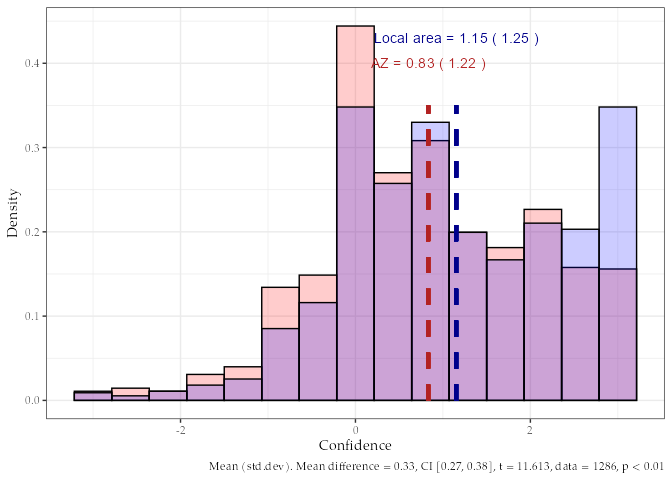
\includegraphics[keepaspectratio]{index_files/figure-latex/notebooks-figures-fig-dist-output-1.png}}

}

\end{figure}%

Overall, the sample expressed more trust in elections relative to
distrust seeing as how the distribution of confidence is largely
positive. However, there's a clear difference between confidence in
Maricopa county, AZ elections and elections within one's local area. A
paired t-test confirms that this difference was statistically
significant, though somewhat small (mean difference \(= 0.325\),
\(95\%\) CI \([0.27, 0.38]\), \(t(1286) = 11.61\), \(p < .001\)).
Nonetheless, respondents appeared less confident regarding elections in
Maricopa County, AZ, but held more confidence in elections
administration in their local area. This complements previous research
that demonstrates a similar bias favorable to one's local area
(\citeproc{ref-stewart2022}{Stewart 2022}).

Accordingly, when confidence levels are distinguished by experiment
condition, the treatment vignette only had an effect upon survey items
pertaining to elections in Maricopa County, AZ. Conducting an
independent samples t-test (i.e., Welch Two Sample t-test) suggests that
the effect of the treatment compared to the control condition is
positive and statistically significant.

\begin{table}[H]

\caption{\label{tbl-ttest}Mean Difference of Treatment Compared to
Control Condition}

\centering{

\centering
\begin{tblr}[         %% tabularray outer open
]                     %% tabularray outer close
{                     %% tabularray inner open
colspec={Q[]Q[]Q[]Q[]Q[]Q[]Q[]Q[]Q[]Q[]},
column{2,3,4,5,6,7,8,9,10}={}{font=\fontsize{0.75em}{1.05em}\selectfont, halign=c,},
column{1}={}{font=\fontsize{0.75em}{1.05em}\selectfont, halign=l,},
}                     %% tabularray inner close
\toprule
Place & $\bar{x}_{diff}$ & $\bar{x}_{treat}$ & $\bar{x}_{control}$ & $n_{treat}$ & $n_{control}$ & t & p & df & CI \\ \midrule %% TinyTableHeader
Maricopa County, AZ & $0.20$ & $0.93$ & $0.72$ & $650.00$ & $637.00$ & 2.96 & 0.003** & 1283.73 & [ 0.07, 0.33] \\
Local Area & $0.06$ & $1.18$ & $1.12$ & $650.00$ & $637.00$ & 0.87 & 0.383 & 1282.95 & [-0.08, 0.20] \\
\bottomrule
\end{tblr}

}

\end{table}%

The results of Table~\ref{tbl-ttest} show that, on a scale ranging from
-3 to 3, the effect of the treatment is associated with a \(0.20\)
average difference in confidence in elections in Maricopa County, AZ,
compared to the control group. When the dependent variable is centered
to have a mean of \(0\) and standard deviation of \(1\), standardized
parameters permit interpretation of the treatment effect in terms of
standard deviations; the standardized difference in confidence between
treatment and control is \(0.16\) (CI \([0.06, 0.27]\)).

\begin{figure}[H]

\caption{\label{fig-coef1}Confidence in Elections by Experiment
Condition}

\begin{minipage}{\linewidth}

\subcaption{\label{fig-coef1-1}Confidence by Treatment Condition}

\centering{

\pandocbounded{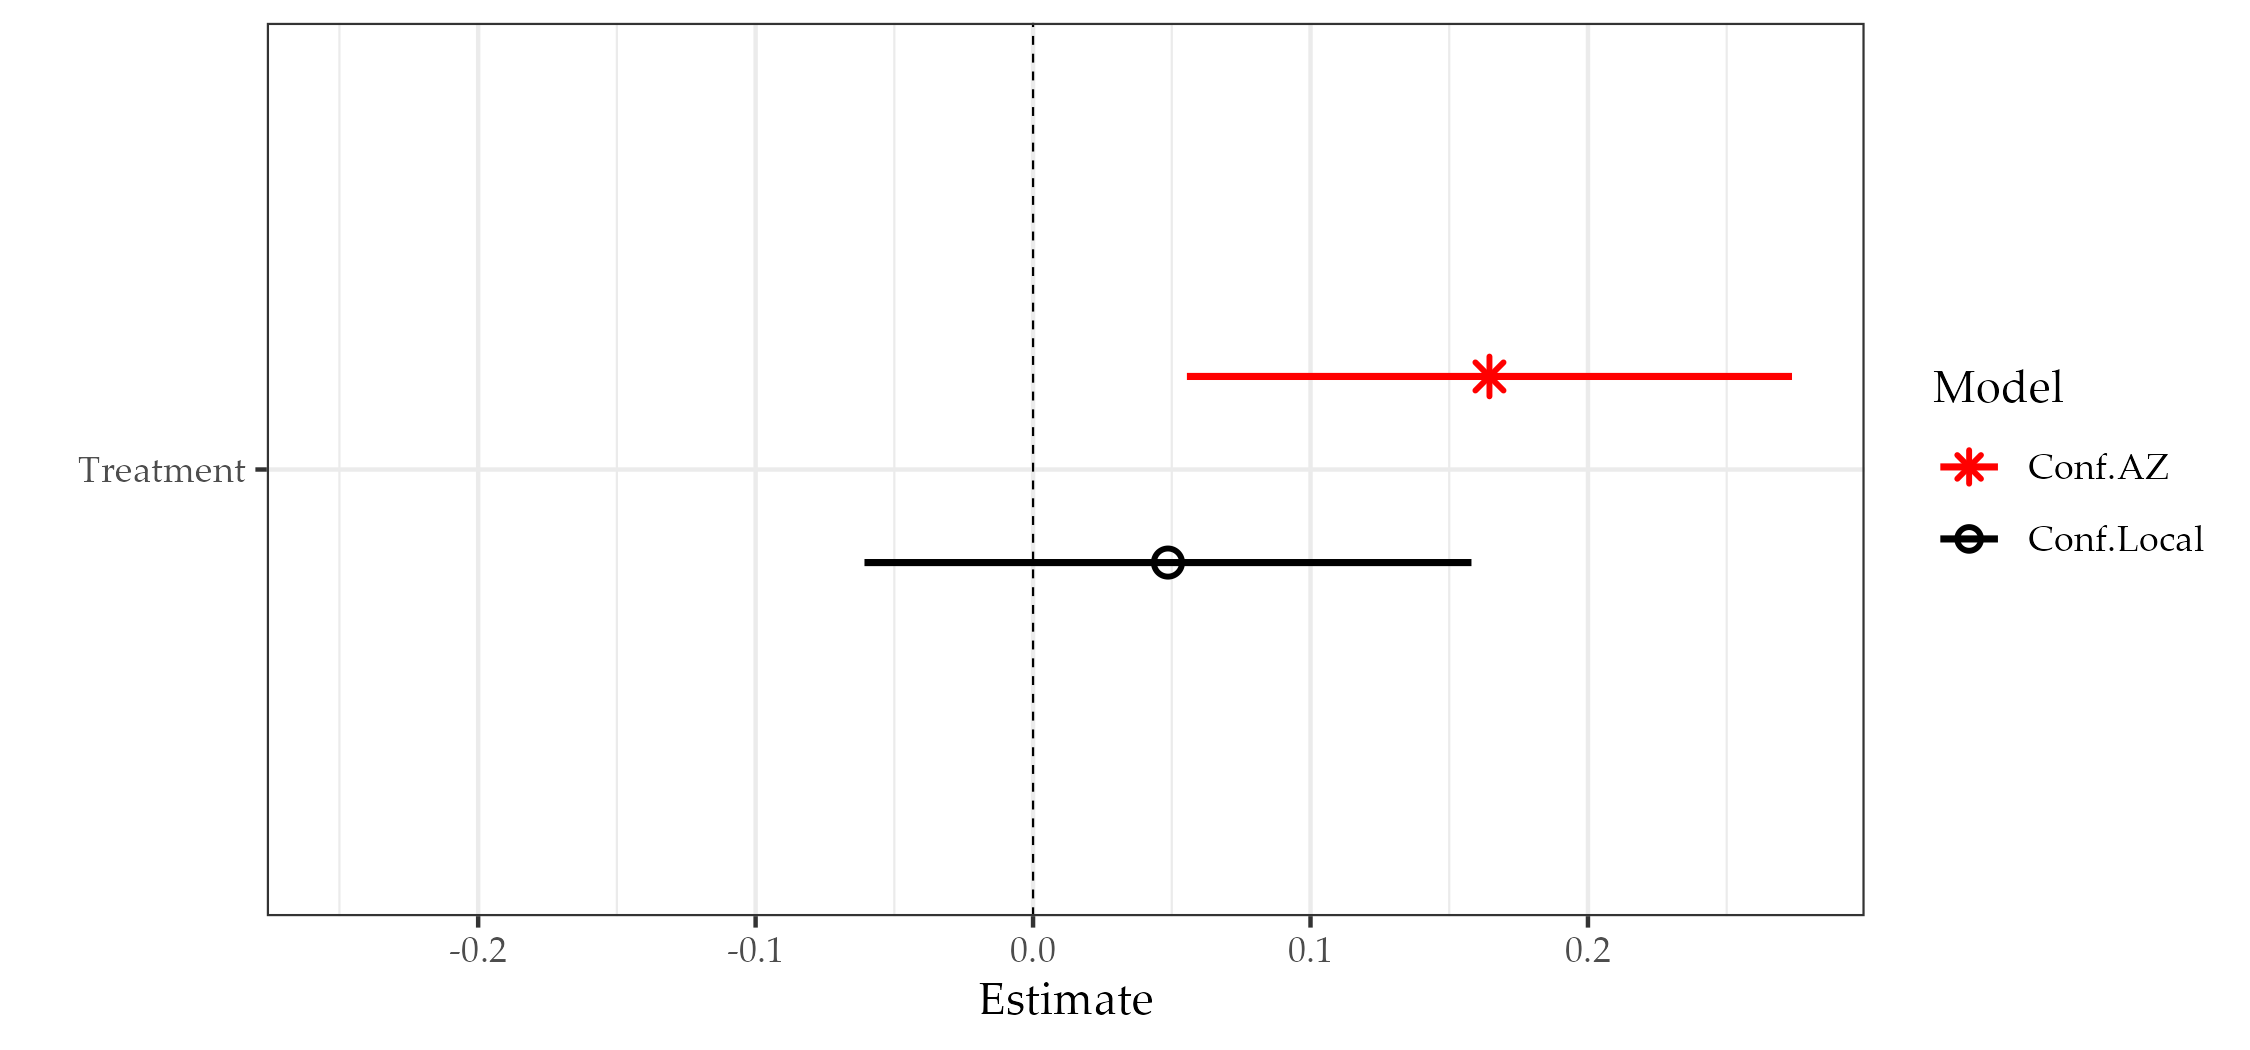
\includegraphics[keepaspectratio]{index_files/figure-pdf/fig-coef1-1.png}}

}

\end{minipage}%
\newline
\begin{minipage}{\linewidth}

\subcaption{\label{fig-coef1-2}Trust and Distrust by Treatment
Condition}

\centering{

\pandocbounded{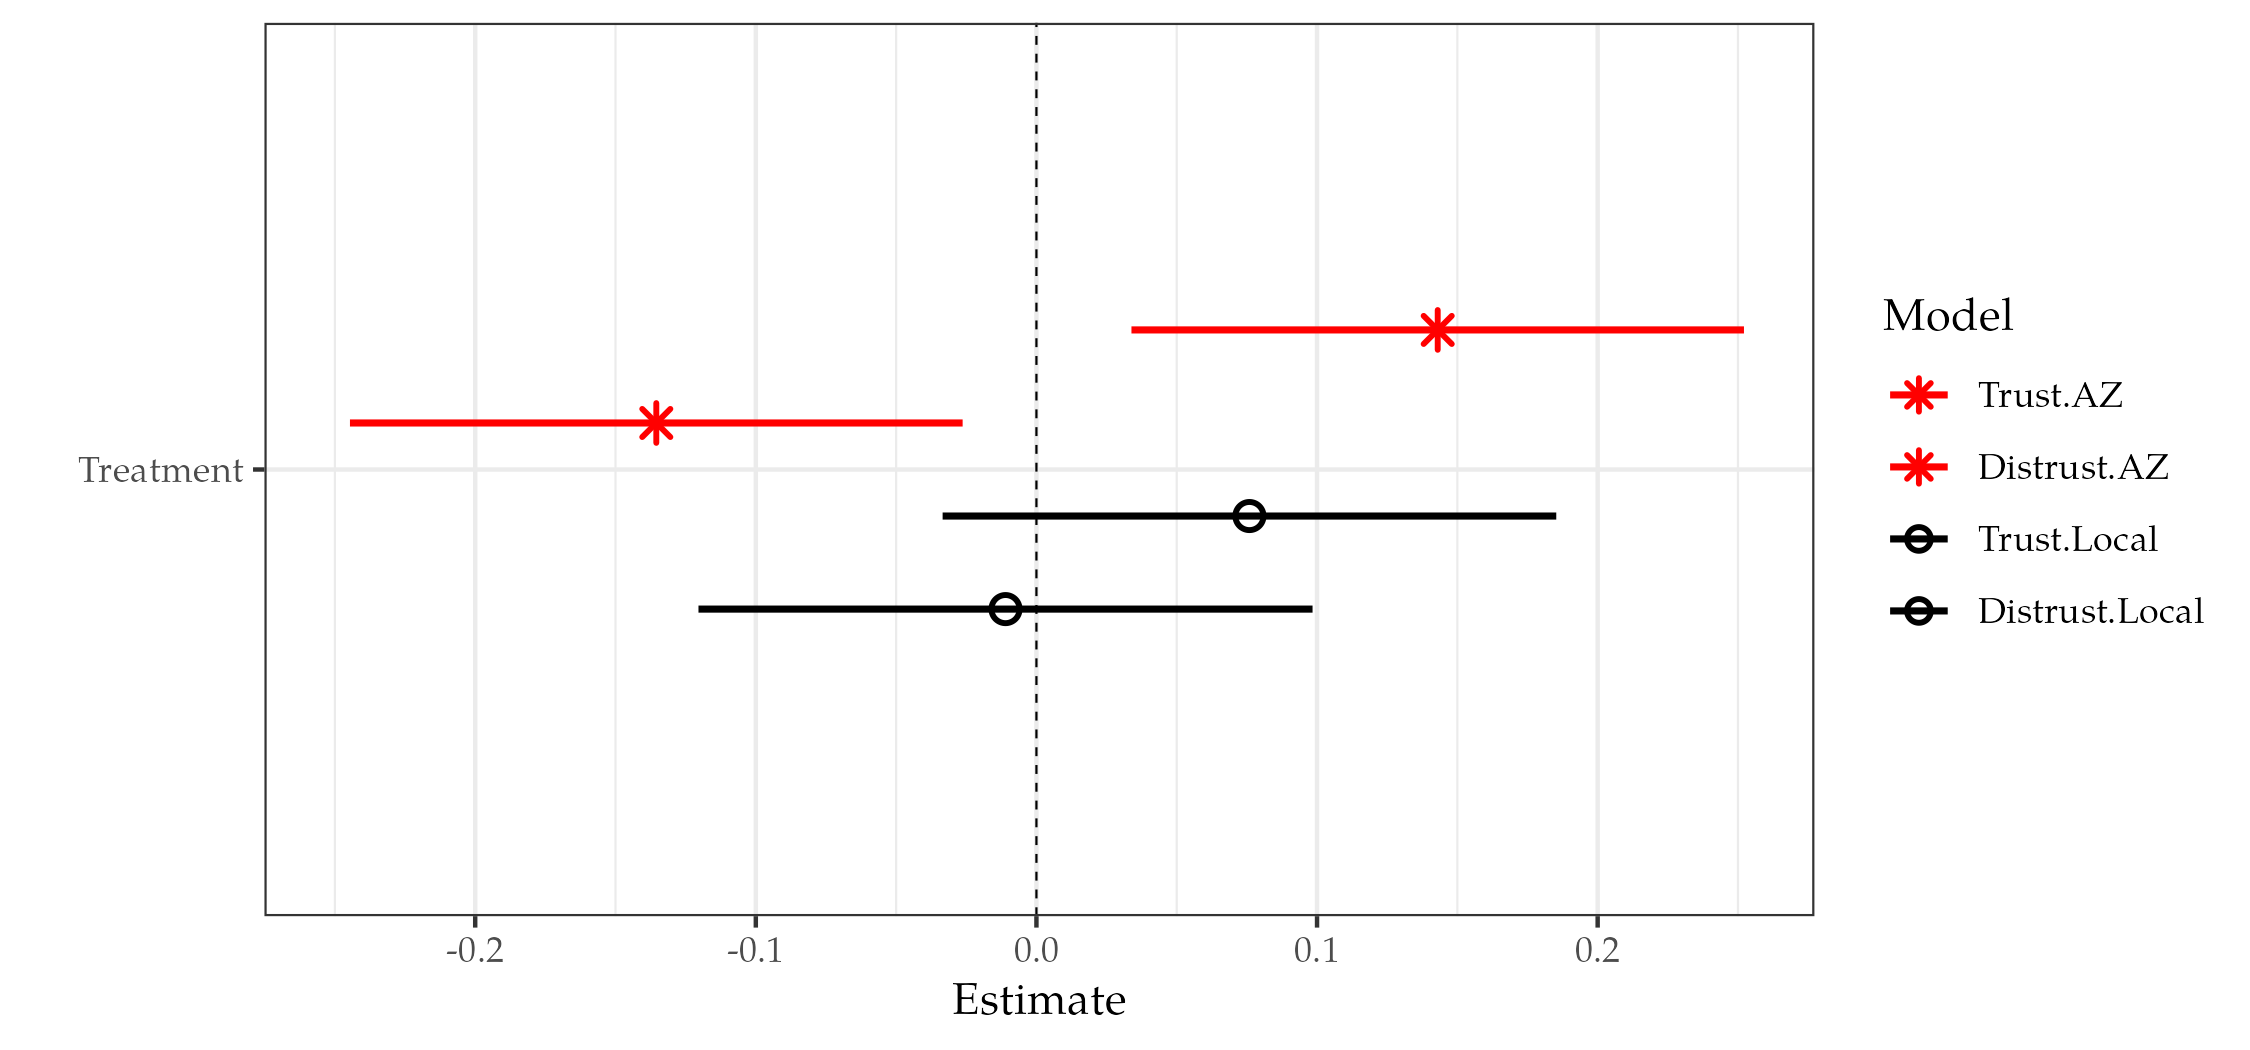
\includegraphics[keepaspectratio]{index_files/figure-pdf/fig-coef1-2.png}}

}

\end{minipage}%

\end{figure}%

Figure~\ref{fig-coef1} displays standard difference estimates of
confidence in elections by treatment condition (control condition as
reference). Figure~\ref{fig-coef1-1} displays two models for confidence
in elections in Maricopa County, AZ, and one's local area by treatment
condition; Figure~\ref{fig-coef1-2} displays the same except
\emph{confidence} is decomposed into its two components, \emph{trust}
and \emph{distrust}. These figures merely illustrate the effect of the
treatment with respect to the relationship between trust and distrust;
ultimately confidence improves.

Confidence in elections was higher among those who read the treatment
vignette but remained conditional on whether the survey questions
inquired about elections in Maricopa County, AZ. This evidence suggests
that announcing efforts to recruit veterans and their families to work
as election staff and volunteers may increase confidence in elections
administration in places outside of one's local area, but may not boost
confidence in elections within one's local area.

The veteran cue is potentially compensatory, which supports the second
hypothesis (H\textsubscript{2}). That is, the gap in confidence in local
elections and elections in Maricopa County is reduced by the veterans
cue, therefore compensating for the otherwise lower confidence and
greater insecurity in Maricopa County elections. This is analogous to
studies showing that Republicans support for a Democratic candidate is
compensated by a Democratic candidate's veteran status. Hypothetical
Democratic veteran candidates were more palatable to Republican
partisans than non-veteran Democrats
(\citeproc{ref-mcdermott2015}{McDermott and Panagopoulos 2015}).
Similarly, Democratic veterans received higher support in Senate races,
especially Democratic veteran Senate candidates whose military
experience included deployment to conflict zones
(\citeproc{ref-richardson2022}{Richardson 2022}).

The point of note is that it is \emph{Democratic} candidates who receive
\emph{more} of a benefit that comes with veteran status\footnote{Note
  that the war veteran classification provided benefits to Republican
  Senate candidates vote share distinct from ``common'' veterans---i.e.,
  Republican Senate candidates who did not deploy to areas of conflict
  (\citeproc{ref-richardson2022}{Richardson 2022}).}; the analogy being
that it is elections located elsewhere that receive the benefits of the
veteran cue whereas local elections do not. Note that the results can't
necessarily be read as differing between elections at the local level
versus national level, but rather heterogeneous effects differ by
elections at the local level and elections in Maricopa County, AZ. The
compensatory effect of the veteran cue may generalize to other
jurisdictions other than one's local area, or the effect may be confined
to Maricopa County, AZ given that this specific county had been made
especially salient in the past.

\subsubsection{2020 Election Legitimacy
Beliefs}\label{election-legitimacy-beliefs}

I now turn to results examining the effect of the treatment on those who
held onto the belief that the 2020 election results were illegitimate.
In short, findings support the third hypothesis (H\textsubscript{3})
allowing me to reject the null. First, reviewing responses to items that
capture trust in elections, it is easy to recognize the difference
between the way 2020 election deniers responded with respect to where
elections were held.

\begin{figure}[!t]

\caption{\label{fig-patch13}Trust in elections by treatment among those
who refute the 2020 election results}

\centering{

\pandocbounded{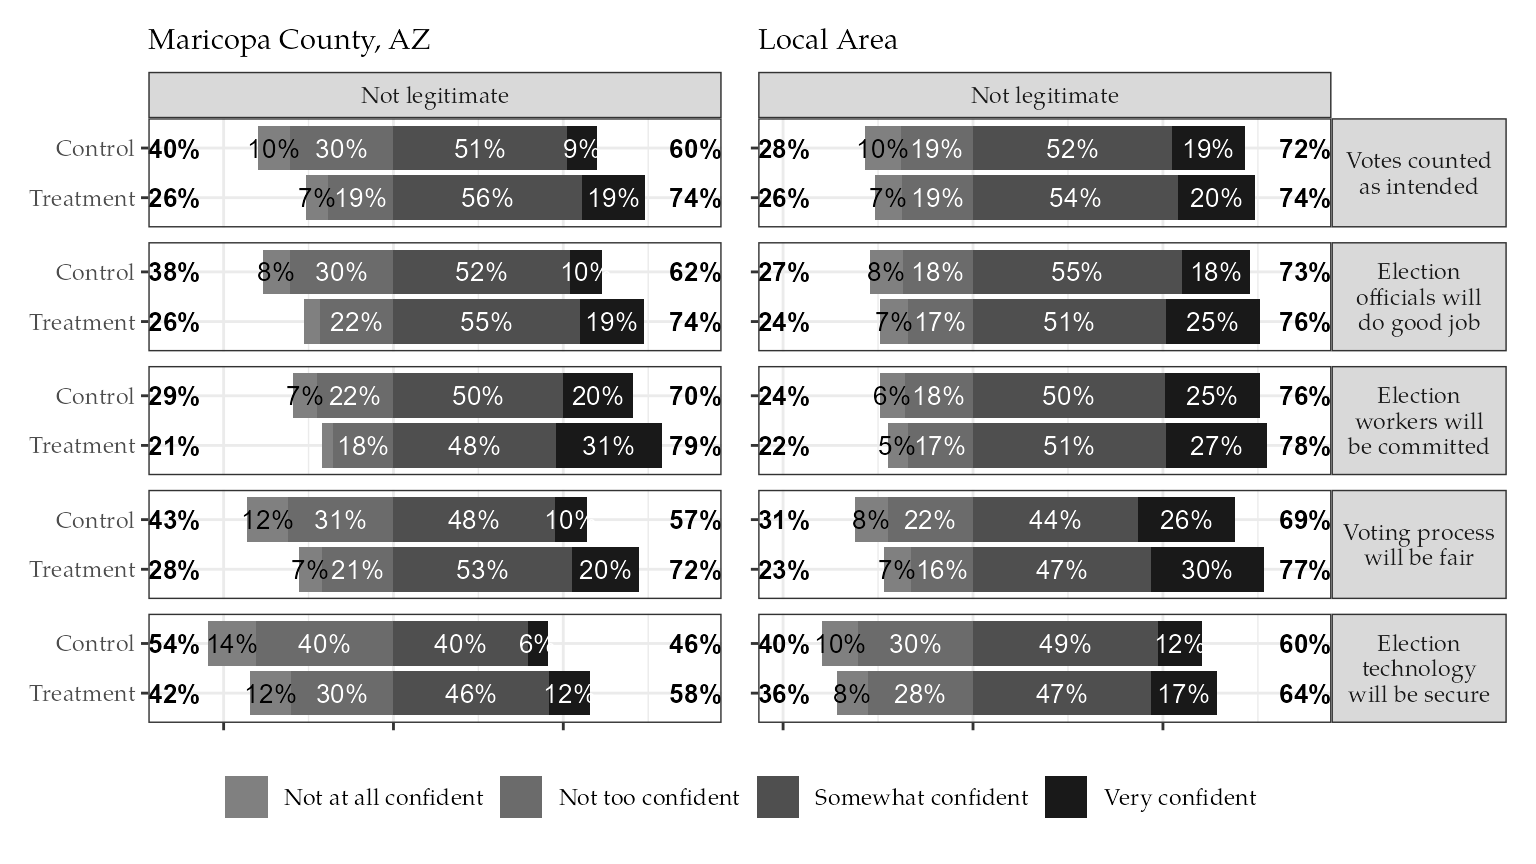
\includegraphics[keepaspectratio]{index_files/figure-latex/notebooks-figures-fig-patch13-output-1.png}}

}

\end{figure}%

Among those who refuted the 2020 election results, trust in Maricopa
County, AZ elections was lower for each item compared to items
pertaining to elections within one's local area, regardless of treatment
condition. However, notably, trust that election technology would be
secure received the lowest confidence endorsement overall. There was
also a notable lack of trust that the voting process would be fair
relative to the other items\footnote{What is interesting to note here is
  that the first three items regard the more human element of the
  election administration process, e.g., ensuring accuracy of counts,
  competence, and commitment of election workers. Although a neat line
  can't really be drawn between the first three and latter two items
  presented here, it is interesting to see a slight divergence from the
  usual high confidence placed in local area elections.}. Now the
comparative difference in responses between those in the treatment group
compared to those in the control group appears substantial for items
pertaining to elections in Maricopa County, AZ.

\begin{figure}[!t]

\caption{\label{fig-patch14}Distrust in elections by treatment among
those who refute the 2020 election results}

\centering{

\pandocbounded{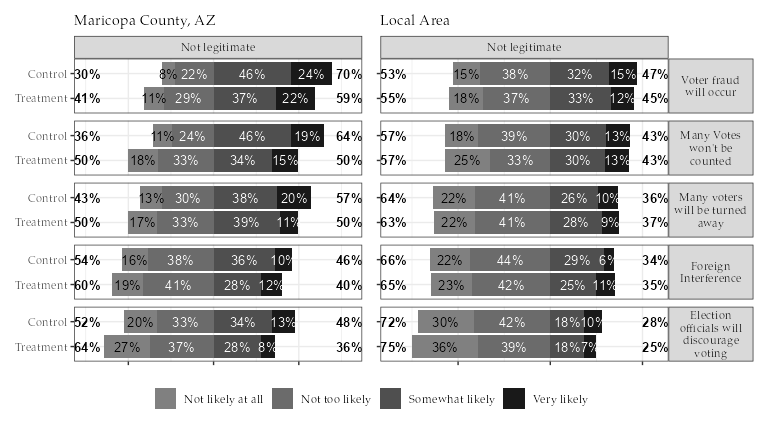
\includegraphics[keepaspectratio]{index_files/figure-latex/notebooks-figures-fig-patch14-output-1.png}}

}

\end{figure}%

Concerning distrust among those who refuted the 2020 election results,
responses to items assessing one's expectation that election fraud would
occur reveal the same pattern. Although there is not as stark a
disparity between responses of those in the treatment and those in the
control, among those in the treatment group, there does appear to be
less expectation that election fraud would occur in Maricopa County, AZ.
Overall, review of responses to trust (Figure~\ref{fig-patch13}) and
distrust survey items (Figure~\ref{fig-patch14}) does lend credence to
the impact of the treatment.

\newpage{}

In order to substantiate the overall influence of the treatment on
confidence in elections, I regressed the dependent variable confidence
on legitimacy beliefs while controlling for partisanship.

\begin{table}[t]

\caption{\label{tbl-legit}Confidence in Elections by Treatment and
Legitimacy Beliefs}

\centering{

\centering
\begin{talltblr}[         %% tabularray outer open
entry=none,label=none,
note{}={{\fontsize{0.75em}{0.75em}\selectfont Outcome variable mean-centered and scaled by 1 standard deviation}},
note{ }={{\fontsize{0.75em}{0.75em}\selectfont + p < 0.1, * p < 0.05, ** p < 0.01, *** p < 0.001}},
]                     %% tabularray outer close
{                     %% tabularray inner open
width={0.8\linewidth},
colspec={X[]X[]X[]},
column{2,3}={}{halign=c, font=\fontsize{0.8em}{1.1em}\selectfont, halign=c,},
column{1}={}{halign=l, font=\fontsize{0.8em}{1.1em}\selectfont, halign=l,},
hline{7}={1,2,3}{solid, black, 0.1em},
}                     %% tabularray inner close
\toprule
& Confidence in AZ Elections & w/Interaction \\ \midrule %% TinyTableHeader
(Intercept) & \num{0.03} (\num{0.08}) & \num{0.07} (\num{0.08}) \\
Treatment & \num{0.18} (\num{0.05})*** & \num{0.09} (\num{0.06}) \\
Not Legitimate & \num{-0.72} (\num{0.07})*** & \num{-0.86} (\num{0.09})*** \\
Republican & \num{0.11} (\num{0.08}) & \num{0.12} (\num{0.08}) \\
Democrat & \num{0.17} (\num{0.09})+ & \num{0.17} (\num{0.09})* \\
Treatment:Not Legitimate &  & \num{0.27} (\num{0.11})* \\
Num.Obs. & \num{1263} & \num{1263} \\
R2 Adj. & \num{0.134} & \num{0.138} \\
\bottomrule
\end{talltblr}

}

\end{table}%

The first model in Table~\ref{tbl-legit} shows that overall confidence
in elections among those who read the treatment vignette was
significantly (statistically) greater than those who read the control,
on average and netting out the effects of partisanship and legitimacy
beliefs. Democratic partisanship remains marginally significant at
\(90\%\) confidence level (\(p = 0.055\)) compared to the reference
group (Independents). Not believing the 2020 election of Joe Biden was
legitimate is negatively associated with confidence in elections. In
order to assess the magnitude of this interaction effect of the
treatment on those who refuted the 2020 election results, I ran a model
where confidence in elections was regressed on the interaction between
the treatment and legitimacy beliefs, controlling for partisanship.

There's a positive interaction effect of the treatment vignette among
those who believe that the 2020 election was not legitimate, on average
and controlling for partisanship. This shows that the treatment effect
was most influential upon those who believe the 2020 election results
were illegitimate. The treatment alone does not reverse such beliefs,
but this shows where its influence was most potent.

\subsubsection{Concerns for Violence and Voter
Safety}\label{concerns-for-violence-and-voter-safety}

While confidence in elections is one concern, it is not the only concern
that arises in anticipation of US elections; the public must feel
confident that voters are safe to cast a ballot in person. The survey
included questions\footnote{See Table~\ref{tbl-6} in Appendix A} that
allowed me to assess whether those in the treatment condition expressed
less concern for violence and more confidence in voter safety compared
to those in the control condition.

\begin{figure}[!t]

\caption{\label{fig-safety-bars}Safety Concerns and Confidence by
Treatment Condition}

\begin{minipage}{\linewidth}

\subcaption{\label{fig-safety-bars-1}Concern for Violence while voting
in Maricopa County, AZ Elections}

\centering{

\pandocbounded{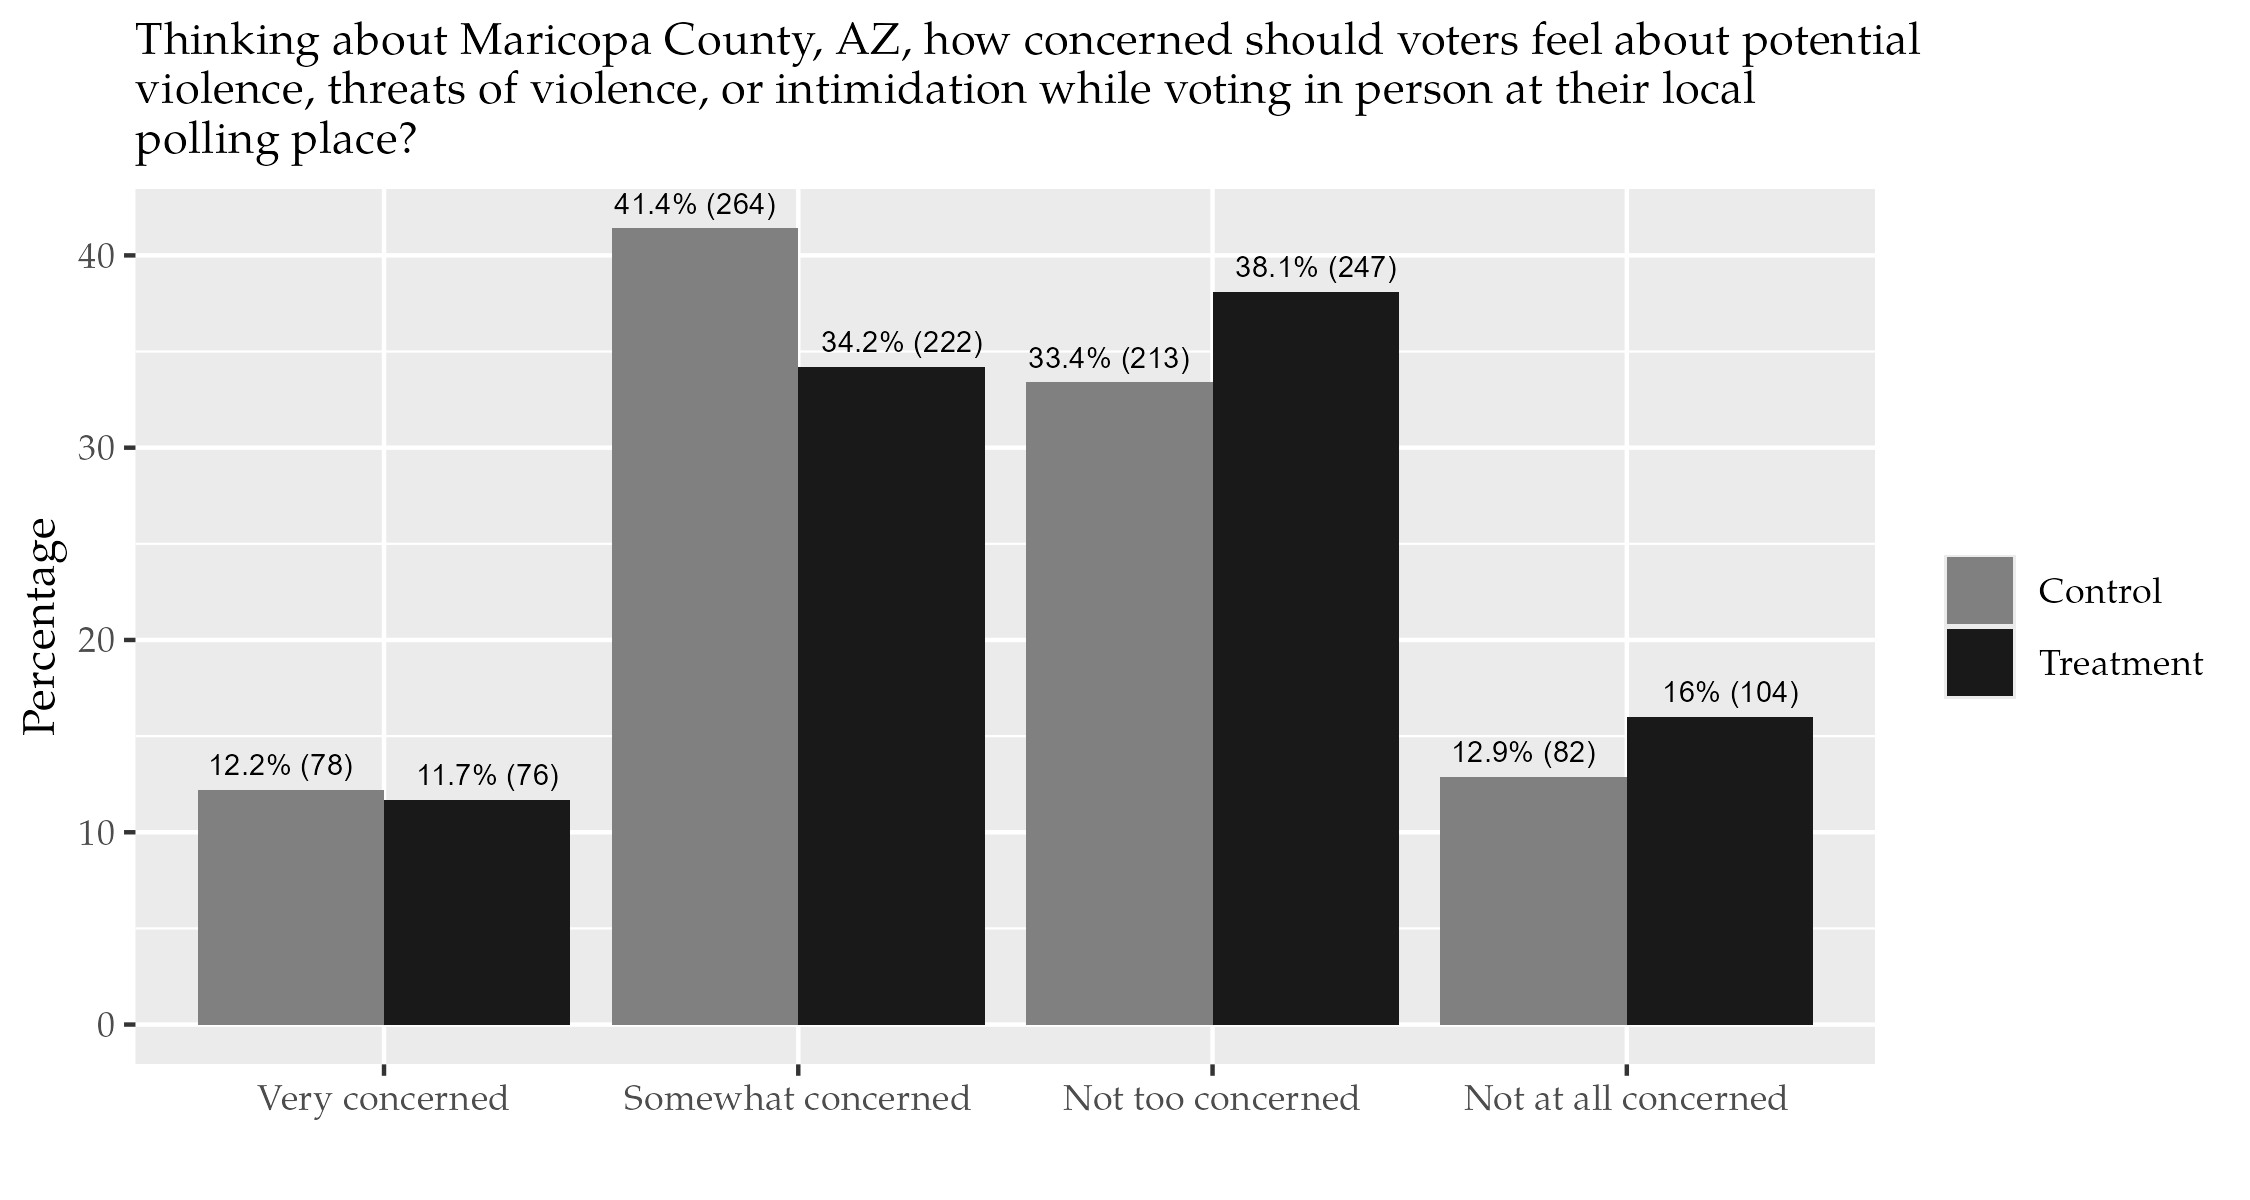
\includegraphics[keepaspectratio]{index_files/figure-pdf/fig-safety-bars-1.png}}

}

\end{minipage}%
\newline
\begin{minipage}{\linewidth}

\subcaption{\label{fig-safety-bars-2}Confidence in Voter Saftey at
Election Sites in Maricopa County, AZ}

\centering{

\pandocbounded{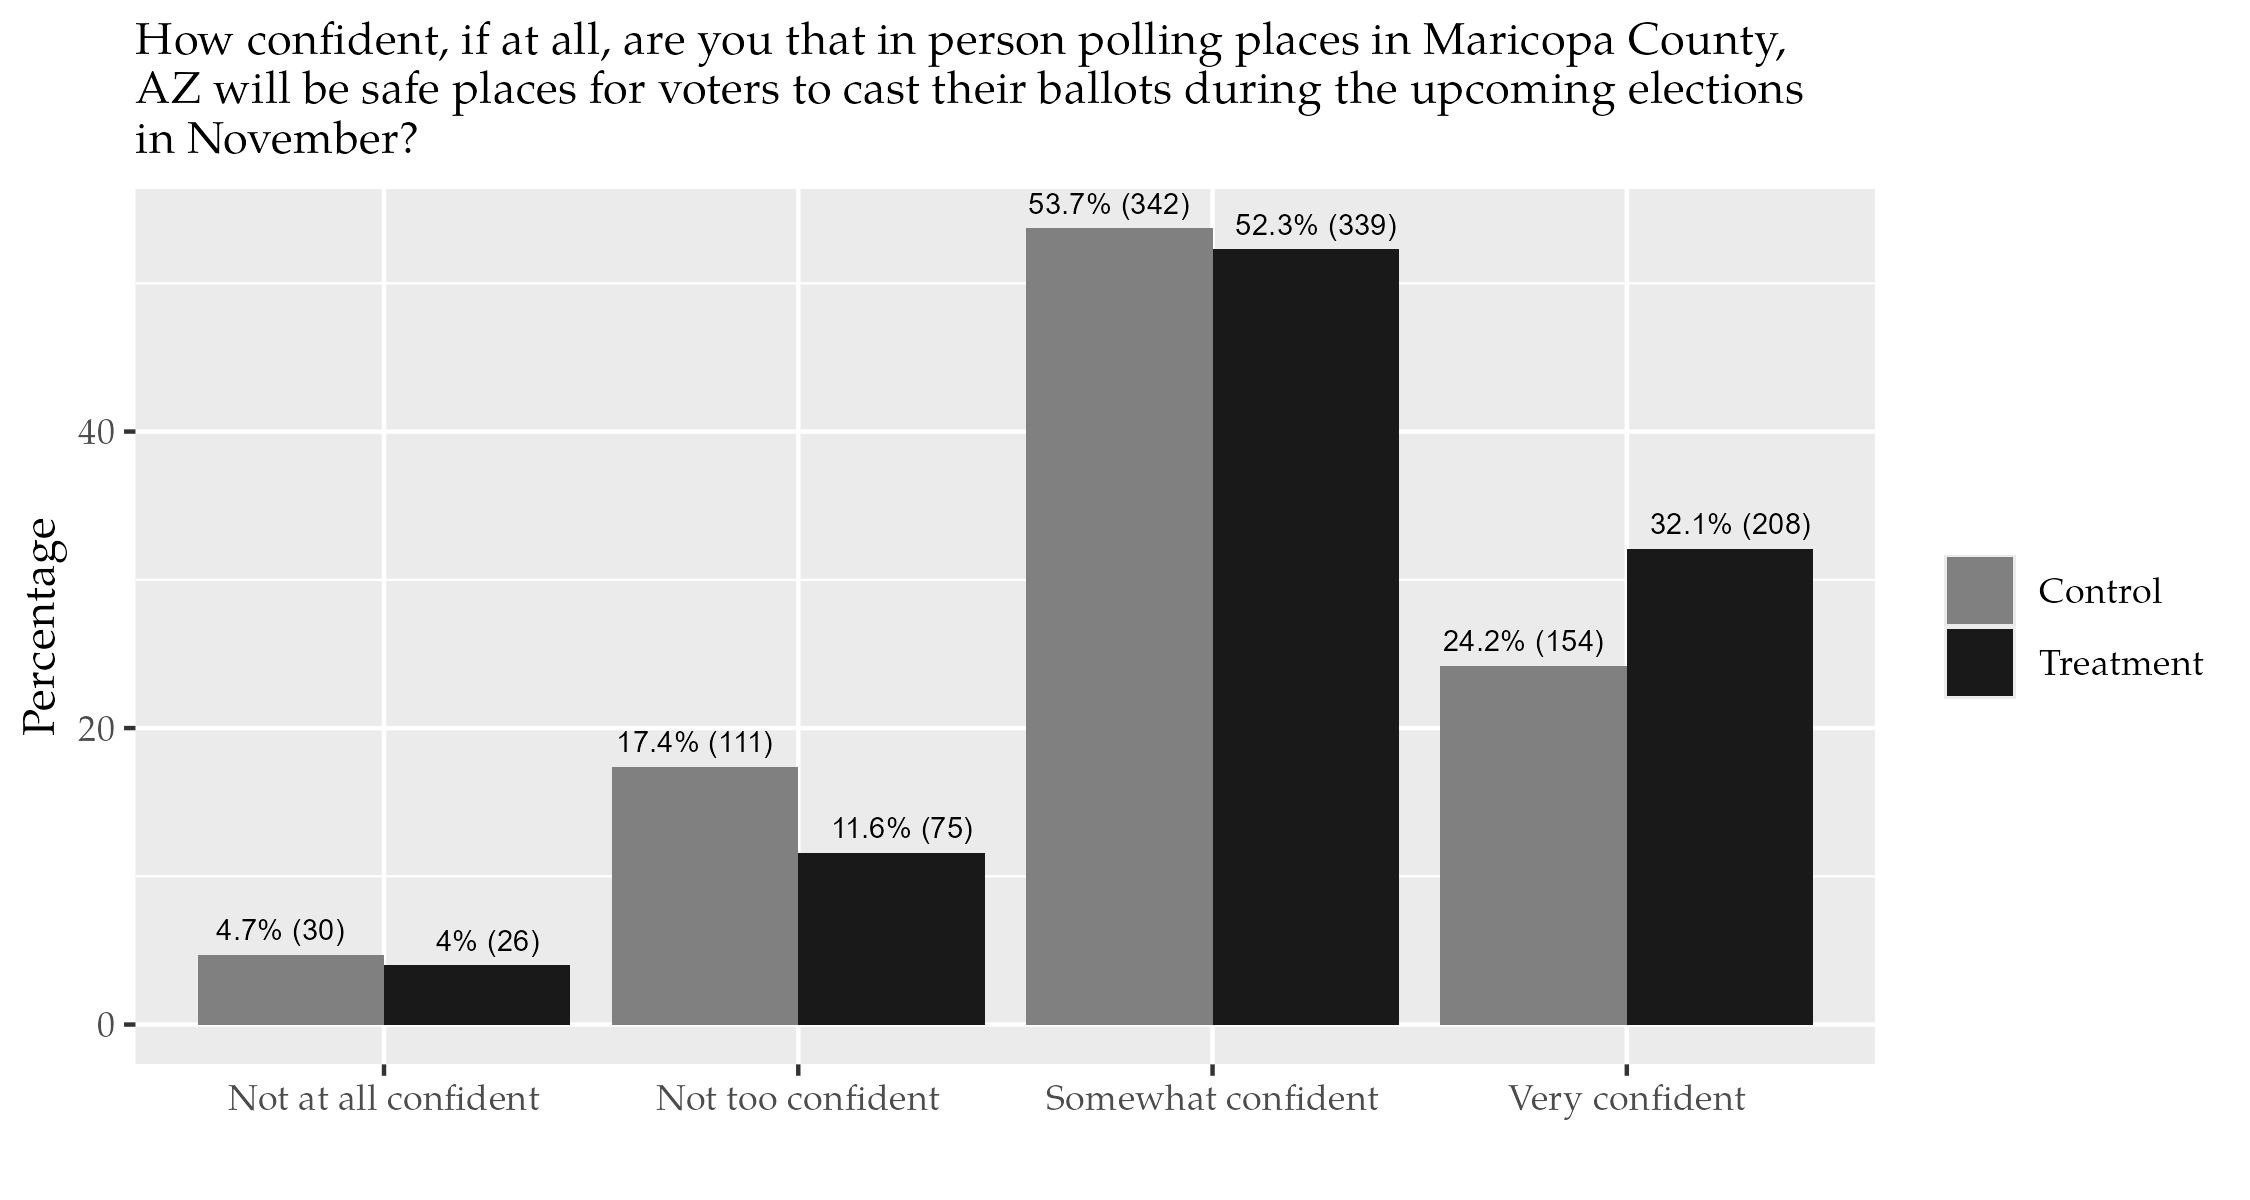
\includegraphics[keepaspectratio]{index_files/figure-pdf/fig-safety-bars-2.png}}

}

\end{minipage}%

\end{figure}%

Briefly reviewing Figure~\ref{fig-safety-bars}, those in the treatment
condition felt less concern over the potential for violence compared to
those in the control. As for confidence in voter safety at election
sites, it appears that more respondents in the treatment condition
expressed that they were ``Very confident'' compared to those in the
control, by approximately \(8\) percentage points.

\newpage{}

It would appear that the treatment vignette increased the likelihood
that a respondent would select a higher response option compared to
those in the control group. In order to assess whether that was the
case, I conducted an ordered logistic regression on the relevant items
using the experimental condition as a dichotomous predictor.

Those in the treatment condition had lower probability to express that
they were `Very' or `Somewhat' concerned for violence in Maricopa
County, AZ Elections, yet higher probability of expressing `Not too' or
`Not at all' concerned. As for confidence in voter safety, moving from
treatment to control, the difference in predicted probability of a
respondent selecting ``Very Confident'' was \(0.08\).
Table~\ref{tbl-preds-diff1} and Table~\ref{tbl-preds-diff2} show the
significant differences in predicted probabilities at 95\(\%\)
confidence\footnote{The same models were run for items pertaining to
  safety concerns in one's local area but results of the treatment were
  not significantly different from the control. See Appendix E for full
  results table of ordinal logistic regression}. These findings support
both H\textsubscript{4a} and H\textsubscript{4b} respectively,
permitting rejection of the null for each hypothesis.

\begin{table}[t]

\caption{\label{tbl-preds-diff1}Difference in Predicted Probabilities in
Concern for violence, Threats of Violence, or Intimidation between
Treatment and Control}

\centering{

\centering
\begin{talltblr}[         %% tabularray outer open
entry=none,label=none,
note{}={{\fontsize{0.75em}{0.75em}\selectfont Results derived from proportional odds logistic regression model. Estimates are differences in predicted probabilities transformed from log odds ratios, and represent difference in estimated prediction of choosing a particular response or higher}},
]                     %% tabularray outer close
{                     %% tabularray inner open
colspec={Q[]Q[]Q[]Q[]Q[]Q[]Q[]},
column{2,3,4,5,6,7}={}{font=\fontsize{0.8em}{1.1em}\selectfont, halign=c,},
column{1}={}{font=\fontsize{0.8em}{1.1em}\selectfont, halign=l,},
}                     %% tabularray inner close
\toprule
Violence & hypothesis & estimate & std.error & z & Pr(>|z|) & conf.int \\ \midrule %% TinyTableHeader
Very concerned & (Treatment) - (Control) & -0.027 & 0.011 & -2.463 & 0.014 & [-0.048, -0.005] \\
Somewhat concerned & (Treatment) - (Control) & -0.037 & 0.015 & -2.468 & 0.014 & [-0.066, -0.008] \\
Not too concerned & (Treatment) - (Control) & 0.032 & 0.013 & 2.460 & 0.014 & [ 0.007,  0.058] \\
Not at all concerned & (Treatment) - (Control) & 0.031 & 0.013 & 2.472 & 0.013 & [ 0.006,  0.056] \\
\bottomrule
\end{talltblr}

}

\end{table}%

\begin{table}[t]

\caption{\label{tbl-preds-diff2}Difference in Predicted Probabilities in
Confidence that voters will be safe to vote in-person between Treatment
and Control}

\centering{

\centering
\begin{talltblr}[         %% tabularray outer open
entry=none,label=none,
note{}={{\fontsize{0.75em}{0.75em}\selectfont Results derived from proportional odds logistic regression model. Estimates are differences in predicted probabilities transformed from log odds ratios, and represent difference in estimated prediction of choosing a particular response or higher}},
]                     %% tabularray outer close
{                     %% tabularray inner open
colspec={Q[]Q[]Q[]Q[]Q[]Q[]Q[]},
column{2,3,4,5,6,7}={}{font=\fontsize{0.8em}{1.1em}\selectfont, halign=c,},
column{1}={}{font=\fontsize{0.8em}{1.1em}\selectfont, halign=l,},
}                     %% tabularray inner close
\toprule
Voter Safety & hypothesis & estimate & std.error & z & Pr(>|z|) & conf.int \\ \midrule %% TinyTableHeader
Not at all confident & (Treatment) - (Control) & -0.0166 & 0.0048 & -3.4331 & 0.0006 & [-0.0260, -0.0071] \\
Not too confident & (Treatment) - (Control) & -0.0444 & 0.0120 & -3.6929 & 0.0002 & [-0.0680, -0.0208] \\
Somewhat confident & (Treatment) - (Control) & -0.0198 & 0.0066 & -3.0095 & 0.0026 & [-0.0327, -0.0069] \\
Very confident & (Treatment) - (Control) & 0.0808 & 0.0215 & 3.7637 & 0.0002 & [ 0.0387,  0.1228] \\
\bottomrule
\end{talltblr}

}

\end{table}%

\newpage{}

\subsection{Discussion}\label{discussion}

It should be noted that these results are limited to one's expectations
in anticipation of election night. Whether the increase in confidence is
sustained post-election night cannot be inferred from these results.
Moreover, It is yet unclear whether actually encountering and
interacting with veterans working as staff or volunteers at election
sites does much to improve voter confidence after election night
compared to anyone else. It may be the case that assumptions that
veterans are filling spots as election workers and volunteers simply
primes positive expectations as one heads into an election site,
potentially improving voters perceptions of their own experience on the
way out. Further research would be needed to test such an idea.

As stated previously, the survey was fielded on a non-probability sample
of 1,287 U.S. citizens 18 years of age or older. The results presented
here are not assumed to be generalizable to the national population. It
may be feasible to weigh the sample to demographics of the population at
the time the survey was fielded, but this is unnecessary for the
experimental purpose of the study. If similar findings complement or
replicate these results, then the expense of drawing samples more
representative of the national population may be justified. At this
stage, however, the results are limited to demonstrating treatment
effects that are sample dependent.

Note also that the measurement items of the components trust and
distrust, and the method of computing scores for the dependent variable,
confidence in elections, are unique to this study but falls under the
methodological framework of Classical Test Theory (CTT). Although survey
measurement items were either directly drawn from or inspired by similar
survey items found in various other surveys (e.g., SPAE, Pew), the
question wording, response choices, coding, and computation of sum
scores of the dependent variable are specific, thus rendering
measurement of the hypothetical constructs of interest (i.e., trust,
distrust) less comparable across similar studies that profess
measurement of similar constructs (\citeproc{ref-widaman2024}{Widaman
and Revelle 2024}). Namely, trust, distrust, or confidence in elections
as defined and measured here.

It is difficult to compare magnitude of effect with other studies given
that the item number, item wording, measurement, and computation of
confidence in elections is unique across most individual studies to
include this one. For instance, Gaudette et al.
(\citeproc{ref-gaudette2025}{2025}) doesn't compose multiple items into
a single composite measure, but subtracts pre-treatment values from
post-treatment values for single-item measures with Likert-style
response options. Whereas Clayton and Willer
(\citeproc{ref-clayton2023}{2023}) develops a scale referred to as
``Trust in American electoral process'' by taking the mean from three
items. The item wording of that scale is markedly similar to the items
used to compose the trust scale of this study, but the range of response
options differs considerably. Thus, while most studies examining public
confidence in elections often include the core question ``How confidence
are you that your vote {[}will be/was{]} counted as you intended in the
most recent election?'', the different ways that researchers measure and
compute variable scores on the outcome are most often, and
unfortunately, sample dependent. The study of public confidence in
elections is in desperate need of a standard method of measurement, or
even a screened and validated item bank, and this study may be seen as a
baby step to that end.

That being said, this study generally emulates treatment effects of
comparable studies in the literature. Gaudette et al.
(\citeproc{ref-gaudette2025}{2025}) found positive effects of official
messaging from election officials on various items measuring trust in
elections and expectations of electoral fraud. Similarly, Clayton and
Willer (\citeproc{ref-clayton2023}{2023}), confined to a sample of
Republican participants, found positive influence on perceptions of 2020
election legitimacy and trust in the American electoral process from
official messaging by Republican politicians reaffirming the 2020
election results.

The setting of the vignette and specified in survey items might raise
additional concerns on whether results are generalizable. Naming a
specific county in the vignette adds in a potentially influential factor
unaccounted for in the survey; some people may have attitudes about the
county in question, others won't, while others may be muffed to consider
a random county in the U.S. they know nothing about. Naming a real and
somewhat salient county potentially undermines confidence that the
treatment effects are solely attributable to veterans to an unknown
degree. Simply put, there may be something special about Maricopa
County, AZ in particular that generalizes across attitudes of trust or
distrust in elections.

Arguably, however, Maricopa County is indicated as the setting in both
the treatment and control vignettes, thus the only actual difference
between conditions is constrained to the target group being recruited.
Future research may employ vignettes naming a fictional U.S. county to
hopefully eliminate the setting as a concern. Alternatively additional
survey items that ask directly about one's knowledge or sentiment about
the county in question could inform researchers on whether the named
county imposes any undue influence at all, or whether the setting is
associated with other factors such as partisanship.

The data of the current study is limited in helping to discern whether
the treatment garners greater confidence in elections uniformly across
different racial or ethnic groups given that the largest proportion of
the sample identified their race as White (77\%). It is reasonable to
suspect that the treatment vignette might differ by race and ethnicity,
but the sample is insufficient to make such generalizations.
Nevertheless, attitudes about veterans that differ by group may play an
important role in determining whether publicized efforts to recruit
military veterans boosts confidence in elections uniformly or whether
the effect is merely partial to certain segments of the population. In
their research examining whether groups differed in attitudes about
veterans, Kleykamp, Hipes, and MacLean
(\citeproc{ref-kleykamp2018}{2018}) could only speculate as to why
levels of support were lowest among Hispanic and Black respondents.
Other research has found that attitudes about the U.S. military
generally---though not about active or veteran military service members
in particular---differs by race and ethnicity to varying extents, but
could not supply reason for one groups' sentiment over another
(\citeproc{ref-nichols2015}{Nichols 2015}).

Other studies have drawn out disparities in public attitudes about
veterans but in ways that are mostly indirect, i.e., without assessing
public regard for veterans directly. One overarching issue is that
there's limited research that differentiates public regard for veteran
and active military service members from the U.S. military as an
institution in general. For instance, some studies assess public regard
for veterans indirectly by examining whether, and to what extent,
endorsement of certain policies differentiate by whether such policies
benefit veterans or the public generally. In one such study, Republican
partisanship was shown to be the most consistent factor associated with
more favorable attitudes on homelessness and PTSD among the veteran
population, but not among the general adult population
(\citeproc{ref-tsai2021}{Tsai et al. 2021}).

Perhaps unsurprisingly, military veterans appear to be uniquely
deserving in the eyes of Republican partisans
(\citeproc{ref-mcdermott2015}{McDermott and Panagopoulos 2015};
\citeproc{ref-richardson2022}{Richardson 2022};
\citeproc{ref-tsai2021}{Tsai et al. 2021}). As such, military veteran
status may qualify favorable attitudes among Republican partisans
whereas their regard for other non-veteran groups might otherwise
express contempt or indifference. This further indicates a need for
research to determine an underlying mechanism explaining why veterans
incur special favor.

The bluntness of the experimental stimulus and survey items don't allow
us to establish exactly what it is about military veterans in particular
that cues stronger confidence in elections. No survey items assessed
public attitudes about military veterans specifically, pre- nor
post-treatment. This unfortunately leaves no room for me to postulate
and examine any potential mechanisms underlying results. As such, a
question lingers about whether some antecedent mechanism transmits
(i.e., mediates) the effects of the veteran treatment vignette to the
outcome. To put simply, this study reiterates that there \emph{is}
something special about veterans in particular that elicits greater
confidence in elections, but cannot go further in determining exactly
\emph{what} that special something might be.

Factors that \emph{moderate} the relationship of the treatment on the
outcome of interest are likely plenty, but one can only offer conjecture
of a \emph{mediator} driving results. One potential explanation is that
veterans, and all those who serve in the military, potentially function
as a national symbol. The group is abstract just as the nation is
abstract, and the potency of the veteran group emulates the potency of a
national symbol. Recall Benedict Anderson's
(\citeproc{ref-anderson2006}{2006}) meditation on the Tomb of the
Unknown Soldier, ``\ldots saturated with ghostly \emph{national}
imaginings'' (\citeproc{ref-anderson2006}{2006, 9}, emphasis original).
In various studies, national symbols such as the flag, the national
anthem, or even mere appeal to national identity have potent, yet
variable, effects on different outcomes (\citeproc{ref-butz2009}{Butz
2009}; \citeproc{ref-butz2007}{Butz, Plant, and Doerr 2007};
\citeproc{ref-gangl2016}{Gangl, Torgler, and Kirchler 2016};
\citeproc{ref-kalmoe2016}{Kalmoe and Gross 2016};
\citeproc{ref-kemmelmeier2008}{Kemmelmeier and Winter 2008};
\citeproc{ref-levendusky2018}{M. S. Levendusky 2018};
\citeproc{ref-schatz2007}{Schatz and Lavine 2007}). It is plausible that
military service members and veterans function in much the same way---as
a symbol of national loyalty, pride, and nationalism for people to
praise and revere out of a sense of duty prescribed by social norm and
reinforced by national sentiment. As such, it may be the case that the
treatment effect on confidence in elections is mediated through an
affective response to a national symbol---in this case, veterans. The
veteran cue may indeed stimulate national sentiment and subsequently
boost confidence in elections.

In results presented here, confidence in elections is associated with
greater confidence among those in the treatment group, but neither
vignette conveys information about the procedures or practices meant to
safeguard election integrity; nothing in the treatment suggests to
respondents that election integrity would be improved by recruiting
veterans. Arguably, the results presented here speak to the ``emotional
pathway'' mentioned in Gaudette et al.
(\citeproc{ref-gaudette2025}{2025}) so long as we assume that there's an
inherent appeal to national sentiment (e.g., nationalism, patriotism) by
use of veterans\footnote{The study by Gaudette et al.
  (\citeproc{ref-gaudette2025}{2025}) included an experiment that
  examined the contrast between ``emotional'' versus ``informational''
  appeals on trust in elections and beliefs that election fraud is
  prevalent. Authors presented one of two video messages created by
  election administration officials in either Virginia or Maricopa
  County, AZ; the former was ``emotions-based'' in that it provided
  little to no information about the voting process or election
  administration, whereas the latter provided, ``\ldots specific
  information about the processes used to ensure the integrity of the
  vote with no appeal to emotion or patriotism''
  (\citeproc{ref-gaudette2025}{2025, 13}).}. Importantly, if the
veterans treatment is mediated by stimulation of affect for nation or
national identity, then comparable stimulation of national sentiment
unrelated to veterans should produce similar results via this
``emotional-pathway''. However, appeals to national sentiment by use of
sterile national symbols (e.g., banal presentation of the U.S. flag,
playing of the national anthem) may not have the same affective
influence on confidence in elections.

In a similar vein, it is plausible that certain political apprehensions
are nullified insofar as veterans as a group are generally perceived as
`apolitical'---which itself may be enough to engender favor among the
mass public (\citeproc{ref-krupnikov2022}{Krupnikov and Ryan 2022}).
Current and former military service members may be viewed by the public
generally as `apolitical', especially in comparison to practically any
other social group. Indeed, an `apolitical' reputation has been long
desired by military leaders and top brass (\citeproc{ref-baldor2020}{L.
C. Baldor 2020}; \citeproc{ref-garamone2016}{Garamone 2016b},
\citeproc{ref-garamone2016a}{2016a}; \citeproc{ref-lagrone2019}{LaGrone
2019}) despite evidence to the contrary
(\citeproc{ref-betros2001}{Betros 2001};
\citeproc{ref-mcnerney2006}{Mcnerney 2006}). Nevertheless, the putative
`apolitical' nature of military service may generalize to veteran
service members, and increase confidence in elections based on the
assumption that veterans uphold a commitment to ensure election
integrity above their own personal loyalties, partisanship, or politics.
Prior research has relied on the assumption that such a
``\emph{group-based}'' norm persists among military members, which
prescribes that the military is, or ought to be, apolitical
(\citeproc{ref-mullinix2022}{Mullinix and Lythgoe 2022}). Although, the
extent to which this perception generalizes widely among the mass public
about the military in general, or about current and former service
members in particular, has yet to be examined. Given recent events of
far more overt politicization of the U.S. military
(\citeproc{ref-baldor2025}{L. C. Baldor 2025};
\citeproc{ref-baldor2025a}{L. Baldor 2025b},
\citeproc{ref-baldor2025b}{2025c}, \citeproc{ref-baldor2025c}{2025a};
\citeproc{ref-thomas2025}{Thomas 2025}), it would be useful for future
research to consider whether perceptions about the military generally,
and military leaders in particular, generalize to perceptions about
current and former military service members. Especially insofar as such
attitudes relate to confidence in the electoral process and
administration.

\subsection{Conclusion}\label{conclusion}

Publicized announcements that election officials are actively recruiting
former military service members to work as election staff and volunteers
is associated with greater confidence in elections compared to election
worker recruitment announcements that do not explicitly mention targeted
efforts to recruit former military service members. In addition, such
public announcements eased concerns about violence and increased
confidence that voters would be safe to vote in person at election
sites. Of course, the higher levels of confidence in elections and voter
safety observed among the treatment group were limited to considerations
about elections held in Maricopa County, AZ---presumably beyond one's
local area. This is to be expected bearing in mind that confidence in
elections for one's local area is usually higher than for those beyond.
Thus, there's already more insecurity concerning elections elsewhere for
whatever reason.

One obvious contribution of these results shows that the perceived
trustworthiness of elections administration is amendable to generalized
impressions about the kind and character of the people who work and
volunteer as election staff. Whatever election officials do to boost
public confidence may be overshadowed by impressions about who is
staffing election sites.

In general, public confidence appears strongest when the elections under
consideration regard those within one's local community. Yet, such
strong confidence is not generalized outward to the institution of
elections administration as a whole. Insecurity in the integrity of the
electoral process and its administration may be naturally higher for
elections that occur further from home. Whether that is due to some
local favorability bias or some outward negativity bias is hard to say.
And seeing as how insecurity presents vulnerability, it is perhaps far
easier to inspire a general sense of distrust in the process and its
administration in places more abstract.

In the anticipatory period prior to national elections, publicized
efforts to recruit veterans to work as election staff and volunteers may
be a small, but positive, step towards reducing insecurity in elections
that occur elsewhere. Especially among those who maintained a steadfast
degree of distrust in elections. Despite a lack of evidence that
systematic electoral fraud had occurred in the 2020 election, a
substantial proportion of the population were unwilling to affirm the
legitimacy of the results. However, despite such legitimacy beliefs,
most were not consistent as they expressed varying levels of trust in
different aspects of elections administration. These results say more
about the influence that military veterans have among those who are most
insecure than it does about the public more generally.

\newpage{}

\section{Appendix A: Survey Experiment Vignettes and Survey
Items}\label{appendix-a-survey-experiment-vignettes-and-survey-items}

\subsection{Survey Experiment
Vignettes}\label{survey-experiment-vignettes}

\begin{figure}

\begin{minipage}{0.45\linewidth}

\subsubsection{Treatment Vignette}\label{treatment-vignette-1}

\textbf{Local Military Veterans Recruited for Election Jobs in Maricopa
County}\\
\strut \\
\strut ~~PHOENIX (AP) --- Election officials in Maricopa County,
Arizona, announced a program designed to recruit military veterans and
their family members from the community to serve as election
administrators, including election polling place workers, temporary
workers, and full-time staff. As the U.S. general elections in November
near, election officials must fill several thousand temporary positions
and hundreds of other open positions to ensure sufficient staffing for
the 2024 elections and beyond.\\
\strut \\
\strut ~~Army veteran Jordan Braxton just joined the elections
workforce. Jordan believes their role is important to ensuring a secure,
accurate, and transparent election, ``Many places are short on staff
this election cycle. I served my country in the Army, and I want to do
my part as a veteran and a citizen to ensure that everyone trusts the
process and the outcome of the election.''

\end{minipage}%
%
\begin{minipage}{0.10\linewidth}
~\end{minipage}%
%
\begin{minipage}{0.45\linewidth}

\subsubsection{Control Vignette}\label{control-vignette-1}

\textbf{Local Residents Recruited for Election Jobs in Maricopa
County}\\
\strut \\
\strut ~~PHOENIX (AP) ---Election officials in Maricopa County, Arizona,
announced a program to recruit members of the community to serve as
election administrators, including election polling place workers,
temporary workers, and full-time staff. As the U.S. general elections in
November near, election officials must fill several thousand temporary
positions and hundreds of other open positions to ensure sufficient
staffing for the 2024 elections and beyond.\\
\strut \\
\strut ~~Jordan Braxton just joined the elections workforce. Jordan
believes their role is important to ensuring a secure, accurate, and
transparent election, ``Many places are short on staff this election
cycle. I want to do my part as a citizen to ensure that everyone trusts
the process and the outcome of the election.''

\end{minipage}%

\end{figure}%

\newpage{}

\begin{table}[H]

\caption{\label{tbl-6}Pre-Treatment Survey Items and Response Options}

\centering{

\centering
\begin{tblr}[         %% tabularray outer open
]                     %% tabularray outer close
{                     %% tabularray inner open
width={1\linewidth},
colspec={X[0.7]X[0.3]},
column{1,2}={}{font=\fontsize{0.8em}{1.1em}\selectfont, halign=l,},
}                     %% tabularray inner close
\toprule
Questions & Response \\ \midrule %% TinyTableHeader
Regardless of whom you supported in the 2020 election, do you think Joe Biden's election as president was legitimate, or was he not legitimately elected? & \minipage{\textwidth}\begin{itemize}
\item Legitimate

\item Not legitimate

\end{itemize}\endminipage \\
Thinking about Maricopa County, AZ, how concerned should voters feel about potential violence, threats of violence, or intimidation while voting in person at their local polling place? & \minipage{\textwidth}\begin{itemize}
\item Very concerned

\item Somewhat concerned

\item Not too concerned

\item Not at all concerned

\end{itemize}\endminipage \\
How confident, if at all, are you that in person polling places in Maricopa County, AZ will be safe places for voters to cast their ballots during the upcoming elections in November? & \minipage{\textwidth}\begin{itemize}
\item Not at all confident

\item Not too confident

\item Somewhat confident

\item Very confident

\end{itemize}\endminipage \\
Thinking about your local area, how concerned should voters feel about potential violence, threats of violence, or intimidation while voting in person at their local polling place? & \minipage{\textwidth}\begin{itemize}
\item Very concerned

\item Somewhat concerned

\item Somewhat unconcerned

\item Not at all concerned

\end{itemize}\endminipage \\
How confident, if at all, are you that in person polling places in your local area will be safe places for voters to cast their ballots during the upcoming elections in November? & \minipage{\textwidth}\begin{itemize}
\item Not at all confident

\item Not too confident

\item Somewhat confident

\item Very confident

\end{itemize}\endminipage \\
\bottomrule
\end{tblr}

}

\end{table}%

\newpage{}

\section{Appendix B: Sample Demographics and
Balance}\label{appendix-b-sample-demographics-and-balance}

\subsection{Sample Demographics}\label{sample-demographics}

\begin{table}

\caption{\label{tbl-demog}Sample Demographics}

\centering{

\centering
\begin{tblr}[         %% tabularray outer open
]                     %% tabularray outer close
{                     %% tabularray inner open
colspec={Q[]Q[]Q[]Q[]},
cell{2}{1}={c=4}{},cell{5}{1}={c=4}{},cell{10}{1}={c=4}{},cell{15}{1}={c=4}{},cell{22}{1}={c=4}{},cell{27}{1}={c=4}{},cell{33}{1}={c=4}{},cell{39}{1}={c=4}{},cell{44}{1}={c=4}{},
column{2,3,4}={}{font=\fontsize{0.8em}{1.1em}\selectfont, halign=c,},
cell{1}{1}={}{font=\fontsize{0.8em}{1.1em}\selectfont, halign=l,},
cell{2}{1}={}{font=\fontsize{0.8em}{1.1em}\selectfont, halign=l,},
cell{5}{1}={}{font=\fontsize{0.8em}{1.1em}\selectfont, halign=l,},
cell{10}{1}={}{font=\fontsize{0.8em}{1.1em}\selectfont, halign=l,},
cell{15}{1}={}{font=\fontsize{0.8em}{1.1em}\selectfont, halign=l,},
cell{22}{1}={}{font=\fontsize{0.8em}{1.1em}\selectfont, halign=l,},
cell{27}{1}={}{font=\fontsize{0.8em}{1.1em}\selectfont, halign=l,},
cell{33}{1}={}{font=\fontsize{0.8em}{1.1em}\selectfont, halign=l,},
cell{39}{1}={}{font=\fontsize{0.8em}{1.1em}\selectfont, halign=l,},
cell{44}{1}={}{font=\fontsize{0.8em}{1.1em}\selectfont, halign=l,},
cell{3}{1}={}{preto={\hspace{2em}}, font=\fontsize{0.8em}{1.1em}\selectfont, halign=l,},
cell{4}{1}={}{preto={\hspace{2em}}, font=\fontsize{0.8em}{1.1em}\selectfont, halign=l,},
cell{6}{1}={}{preto={\hspace{2em}}, font=\fontsize{0.8em}{1.1em}\selectfont, halign=l,},
cell{7}{1}={}{preto={\hspace{2em}}, font=\fontsize{0.8em}{1.1em}\selectfont, halign=l,},
cell{8}{1}={}{preto={\hspace{2em}}, font=\fontsize{0.8em}{1.1em}\selectfont, halign=l,},
cell{9}{1}={}{preto={\hspace{2em}}, font=\fontsize{0.8em}{1.1em}\selectfont, halign=l,},
cell{11}{1}={}{preto={\hspace{2em}}, font=\fontsize{0.8em}{1.1em}\selectfont, halign=l,},
cell{12}{1}={}{preto={\hspace{2em}}, font=\fontsize{0.8em}{1.1em}\selectfont, halign=l,},
cell{13}{1}={}{preto={\hspace{2em}}, font=\fontsize{0.8em}{1.1em}\selectfont, halign=l,},
cell{14}{1}={}{preto={\hspace{2em}}, font=\fontsize{0.8em}{1.1em}\selectfont, halign=l,},
cell{16}{1}={}{preto={\hspace{2em}}, font=\fontsize{0.8em}{1.1em}\selectfont, halign=l,},
cell{17}{1}={}{preto={\hspace{2em}}, font=\fontsize{0.8em}{1.1em}\selectfont, halign=l,},
cell{18}{1}={}{preto={\hspace{2em}}, font=\fontsize{0.8em}{1.1em}\selectfont, halign=l,},
cell{19}{1}={}{preto={\hspace{2em}}, font=\fontsize{0.8em}{1.1em}\selectfont, halign=l,},
cell{20}{1}={}{preto={\hspace{2em}}, font=\fontsize{0.8em}{1.1em}\selectfont, halign=l,},
cell{21}{1}={}{preto={\hspace{2em}}, font=\fontsize{0.8em}{1.1em}\selectfont, halign=l,},
cell{23}{1}={}{preto={\hspace{2em}}, font=\fontsize{0.8em}{1.1em}\selectfont, halign=l,},
cell{24}{1}={}{preto={\hspace{2em}}, font=\fontsize{0.8em}{1.1em}\selectfont, halign=l,},
cell{25}{1}={}{preto={\hspace{2em}}, font=\fontsize{0.8em}{1.1em}\selectfont, halign=l,},
cell{26}{1}={}{preto={\hspace{2em}}, font=\fontsize{0.8em}{1.1em}\selectfont, halign=l,},
cell{28}{1}={}{preto={\hspace{2em}}, font=\fontsize{0.8em}{1.1em}\selectfont, halign=l,},
cell{29}{1}={}{preto={\hspace{2em}}, font=\fontsize{0.8em}{1.1em}\selectfont, halign=l,},
cell{30}{1}={}{preto={\hspace{2em}}, font=\fontsize{0.8em}{1.1em}\selectfont, halign=l,},
cell{31}{1}={}{preto={\hspace{2em}}, font=\fontsize{0.8em}{1.1em}\selectfont, halign=l,},
cell{32}{1}={}{preto={\hspace{2em}}, font=\fontsize{0.8em}{1.1em}\selectfont, halign=l,},
cell{34}{1}={}{preto={\hspace{2em}}, font=\fontsize{0.8em}{1.1em}\selectfont, halign=l,},
cell{35}{1}={}{preto={\hspace{2em}}, font=\fontsize{0.8em}{1.1em}\selectfont, halign=l,},
cell{36}{1}={}{preto={\hspace{2em}}, font=\fontsize{0.8em}{1.1em}\selectfont, halign=l,},
cell{37}{1}={}{preto={\hspace{2em}}, font=\fontsize{0.8em}{1.1em}\selectfont, halign=l,},
cell{38}{1}={}{preto={\hspace{2em}}, font=\fontsize{0.8em}{1.1em}\selectfont, halign=l,},
cell{40}{1}={}{preto={\hspace{2em}}, font=\fontsize{0.8em}{1.1em}\selectfont, halign=l,},
cell{41}{1}={}{preto={\hspace{2em}}, font=\fontsize{0.8em}{1.1em}\selectfont, halign=l,},
cell{42}{1}={}{preto={\hspace{2em}}, font=\fontsize{0.8em}{1.1em}\selectfont, halign=l,},
cell{43}{1}={}{preto={\hspace{2em}}, font=\fontsize{0.8em}{1.1em}\selectfont, halign=l,},
cell{45}{1}={}{preto={\hspace{2em}}, font=\fontsize{0.8em}{1.1em}\selectfont, halign=l,},
cell{46}{1}={}{preto={\hspace{2em}}, font=\fontsize{0.8em}{1.1em}\selectfont, halign=l,},
cell{47}{1}={}{preto={\hspace{2em}}, font=\fontsize{0.8em}{1.1em}\selectfont, halign=l,},
cell{48}{1}={}{preto={\hspace{2em}}, font=\fontsize{0.8em}{1.1em}\selectfont, halign=l,},
cell{49}{1}={}{preto={\hspace{2em}}, font=\fontsize{0.8em}{1.1em}\selectfont, halign=l,},
}                     %% tabularray inner close
\toprule
& n & percent & valid percent \\ \midrule %% TinyTableHeader
Experiment Condition &&& \\
Control & 637 & 49.5 & - \\
Treatment & 650 & 50.5 & - \\
Age &&& \\
18-34 & 350 & 27.2 & - \\
35-54 & 480 & 37.3 & - \\
55-74 & 390 & 30.3 & - \\
75-85+ & 67 & 5.2 & - \\
Gender &&& \\
Male & 598 & 46.5 & 47.0 \\
Female & 658 & 51.1 & 51.7 \\
Other/Refused & 16 & 1.2 & 1.3 \\
NA & 15 & 1.2 & - \\
Race &&& \\
White or Caucasian & 975 & 75.8 & 76.7 \\
Black or African American & 164 & 12.7 & 12.9 \\
American Indian & 22 & 1.7 & 1.7 \\
Asian & 56 & 4.4 & 4.4 \\
Other & 55 & 4.3 & 4.3 \\
NA & 15 & 1.2 & - \\
Hispanic, Latino, or Spanish Origin &&& \\
Yes & 113 & 8.8 & 8.9 \\
No & 1148 & 89.2 & 90.3 \\
Prefer not to say & 11 & 0.9 & 0.9 \\
NA & 15 & 1.2 & - \\
Education &&& \\
H.S. or less & 362 & 28.1 & 28.5 \\
Some college no degree & 283 & 22.0 & 22.2 \\
College degree & 461 & 35.8 & 36.2 \\
Postgraduate degree & 166 & 12.9 & 13.1 \\
NA & 15 & 1.2 & - \\
Military Relation &&& \\
Active Duty & 15 & 1.2 & 1.2 \\
Has Family in Military & 362 & 28.1 & 28.5 \\
No Family in Military & 789 & 61.3 & 62.0 \\
Prior Service (Veteran) & 106 & 8.2 & 8.3 \\
NA & 15 & 1.2 & - \\
Party ID &&& \\
Independent & 162 & 12.6 & 12.8 \\
Republican & 540 & 42.0 & 42.6 \\
Democrat & 566 & 44.0 & 44.6 \\
NA & 19 & 1.5 & - \\
Political Ideology &&& \\
Conservative & 412 & 32.0 & 32.5 \\
Liberal & 392 & 30.5 & 30.9 \\
Moderate & 365 & 28.4 & 28.8 \\
Unsure & 98 & 7.6 & 7.7 \\
NA & 20 & 1.6 & - \\
\bottomrule
\end{tblr}

}

\end{table}%

\newpage{}

\section{Appendix C: Test of Random Assignment to Experiment
Condition}\label{appendix-c-test-of-random-assignment-to-experiment-condition}

Table~\ref{tbl-logit} shows results of a logistic regression test of
random assignment to the treatment group. Demographics such as age,
gender, race, educational attainment, and party ID are included as
predictor variables. Note that 19 missing observations were deleted. A
\(\chi^2 = 11.010\), with 15 degrees of freedom and associated p-value
\textgreater{} 0.05 (\(p = 0.75\)) confirms that none of the demographic
predictor variables significantly increased the log-odds---in turn, the
probability---of being assigned to the treatment group.

\begin{table}[H]

\caption{\label{tbl-logit}Logistic Regression of Random Assignment to
Treatment}

\centering{

\centering
\begin{tblr}[         %% tabularray outer open
]                     %% tabularray outer close
{                     %% tabularray inner open
colspec={Q[]Q[]},
cell{2}{1}={c=2}{},cell{6}{1}={c=2}{},cell{9}{1}={c=2}{},cell{15}{1}={c=2}{},cell{19}{1}={c=2}{},
column{2}={}{halign=c, font=\fontsize{0.7em}{1em}\selectfont, halign=c,},
cell{1}{1}={}{halign=l, font=\fontsize{0.7em}{1em}\selectfont, halign=l,},
cell{2}{1}={}{halign=l, font=\fontsize{0.7em}{1em}\selectfont, halign=l,},
cell{6}{1}={}{halign=l, font=\fontsize{0.7em}{1em}\selectfont, halign=l,},
cell{9}{1}={}{halign=l, font=\fontsize{0.7em}{1em}\selectfont, halign=l,},
cell{15}{1}={}{halign=l, font=\fontsize{0.7em}{1em}\selectfont, halign=l,},
cell{19}{1}={}{halign=l, font=\fontsize{0.7em}{1em}\selectfont, halign=l,},
cell{3}{1}={}{halign=l, preto={\hspace{2em}}, font=\fontsize{0.7em}{1em}\selectfont, halign=l,},
cell{4}{1}={}{halign=l, preto={\hspace{2em}}, font=\fontsize{0.7em}{1em}\selectfont, halign=l,},
cell{5}{1}={}{halign=l, preto={\hspace{2em}}, font=\fontsize{0.7em}{1em}\selectfont, halign=l,},
cell{7}{1}={}{halign=l, preto={\hspace{2em}}, font=\fontsize{0.7em}{1em}\selectfont, halign=l,},
cell{8}{1}={}{halign=l, preto={\hspace{2em}}, font=\fontsize{0.7em}{1em}\selectfont, halign=l,},
cell{10}{1}={}{halign=l, preto={\hspace{2em}}, font=\fontsize{0.7em}{1em}\selectfont, halign=l,},
cell{11}{1}={}{halign=l, preto={\hspace{2em}}, font=\fontsize{0.7em}{1em}\selectfont, halign=l,},
cell{12}{1}={}{halign=l, preto={\hspace{2em}}, font=\fontsize{0.7em}{1em}\selectfont, halign=l,},
cell{13}{1}={}{halign=l, preto={\hspace{2em}}, font=\fontsize{0.7em}{1em}\selectfont, halign=l,},
cell{14}{1}={}{halign=l, preto={\hspace{2em}}, font=\fontsize{0.7em}{1em}\selectfont, halign=l,},
cell{16}{1}={}{halign=l, preto={\hspace{2em}}, font=\fontsize{0.7em}{1em}\selectfont, halign=l,},
cell{17}{1}={}{halign=l, preto={\hspace{2em}}, font=\fontsize{0.7em}{1em}\selectfont, halign=l,},
cell{18}{1}={}{halign=l, preto={\hspace{2em}}, font=\fontsize{0.7em}{1em}\selectfont, halign=l,},
cell{20}{1}={}{halign=l, preto={\hspace{2em}}, font=\fontsize{0.7em}{1em}\selectfont, halign=l,},
cell{21}{1}={}{halign=l, preto={\hspace{2em}}, font=\fontsize{0.7em}{1em}\selectfont, halign=l,},
cell{22}{1}={}{halign=l, preto={\hspace{2em}}, font=\fontsize{0.7em}{1em}\selectfont, halign=l,},
cell{23}{1}={}{halign=l, preto={\hspace{2em}}, font=\fontsize{0.7em}{1em}\selectfont, halign=l,},
cell{24}{1}={}{halign=l, preto={\hspace{2em}}, font=\fontsize{0.7em}{1em}\selectfont, halign=l,},
cell{25}{1}={}{halign=l, preto={\hspace{2em}}, font=\fontsize{0.7em}{1em}\selectfont, halign=l,},
cell{26}{1}={}{halign=l, preto={\hspace{2em}}, font=\fontsize{0.7em}{1em}\selectfont, halign=l,},
cell{27}{1}={}{halign=l, preto={\hspace{2em}}, font=\fontsize{0.7em}{1em}\selectfont, halign=l,},
hline{22}={1,2}{solid, black, 0.05em},
}                     %% tabularray inner close
\toprule
& log(OR) \\ \midrule %% TinyTableHeader
\textbf{Age} & \\
35-54 & -0.166, {[}-0.449, 0.116{]} \\
55-74 & -0.154, {[}-0.455, 0.146{]} \\
75-85+ & 0.402, {[}-0.149, 0.972{]} \\
\textbf{Gender} & \\
Female & -0.069, {[}-0.293, 0.154{]} \\
Other/Refused & -0.625, {[}-1.751, 0.419{]} \\
\textbf{Race} & \\
Asian & 0.028, {[}-0.547, 0.605{]} \\
Black & -0.081, {[}-0.429, 0.267{]} \\
Other & 0.054, {[}-0.821, 0.929{]} \\
Hispanic & -0.236, {[}-0.864, 0.382{]} \\
American Indian & 0.501, {[}-0.577, 1.693{]} \\
\textbf{Education} & \\
Some college no degree & -0.103, {[}-0.418, 0.211{]} \\
College degree & -0.164, {[}-0.446, 0.118{]} \\
Postgraduate degree & 0.023, {[}-0.353, 0.400{]} \\
\textbf{Party ID} & \\
Republican & 0.117, {[}-0.242, 0.477{]} \\
Democrat & 0.048, {[}-0.308, 0.404{]} \\
N & 1268 \\
Log.Lik. & -873.349 \\
Deviance & 1746.69809019881 \\
Deviance Null & 1757.70768353601 \\
Chi2 & 11.010 \\
P(\textgreater{}chisq) & 0.752 \\
\bottomrule
\end{tblr}

}

\end{table}%

\newpage{}

\section{Appendix D: Polychoric Item and Score Correlations of Trust and
Distrust}\label{appendix-d-polychoric-item-and-score-correlations-of-trust-and-distrust}

\subsection{Trust and Distrust}\label{trust-and-distrust}

Polychoric correlation is a measure of association between two ordered
categorical variables each assumed to represent (i.e., indicate, be
influenced by) two normally distributed, continuous, latent variables.
Due to the fact that each item is an ordered categorical variable
assumed to represent one of two latent constructs (i.e., trust or
distrust, respectively), I examined polychoric correlations between the
items used to construct each scale. In addition, one set of the trust
and distrust items pertained to Maricopa County, AZ, whereas the other
set of items were identical except that these items pertained to one's
local area.

Since the two sets of items (AZ items and Local items) are, in theory,
supposed to capture the same normally distributed continuous latent
variables, then the polychoric inter-item correlations should be
significantly associated, strong, and in the same direction for the
items that measure trust regardless of whether the items pertain to AZ
or one's local area (likewise for distrust). Simply, trust/distrust in
elections in AZ should strongly and positively be associated with
trust/distrust in elections in one's local area.

Additionally, the items that indicate trust should negatively correlate
with items that indicate distrust. Furthermore, the strength of the
negative correlations between trust and distrust should closely
approximate if not match.

\phantomsection\label{cell-fig-polycor}
\begin{figure}[h]

\caption{\label{fig-polycor}Polychoric Item Correlation Matrix}

\centering{

\pandocbounded{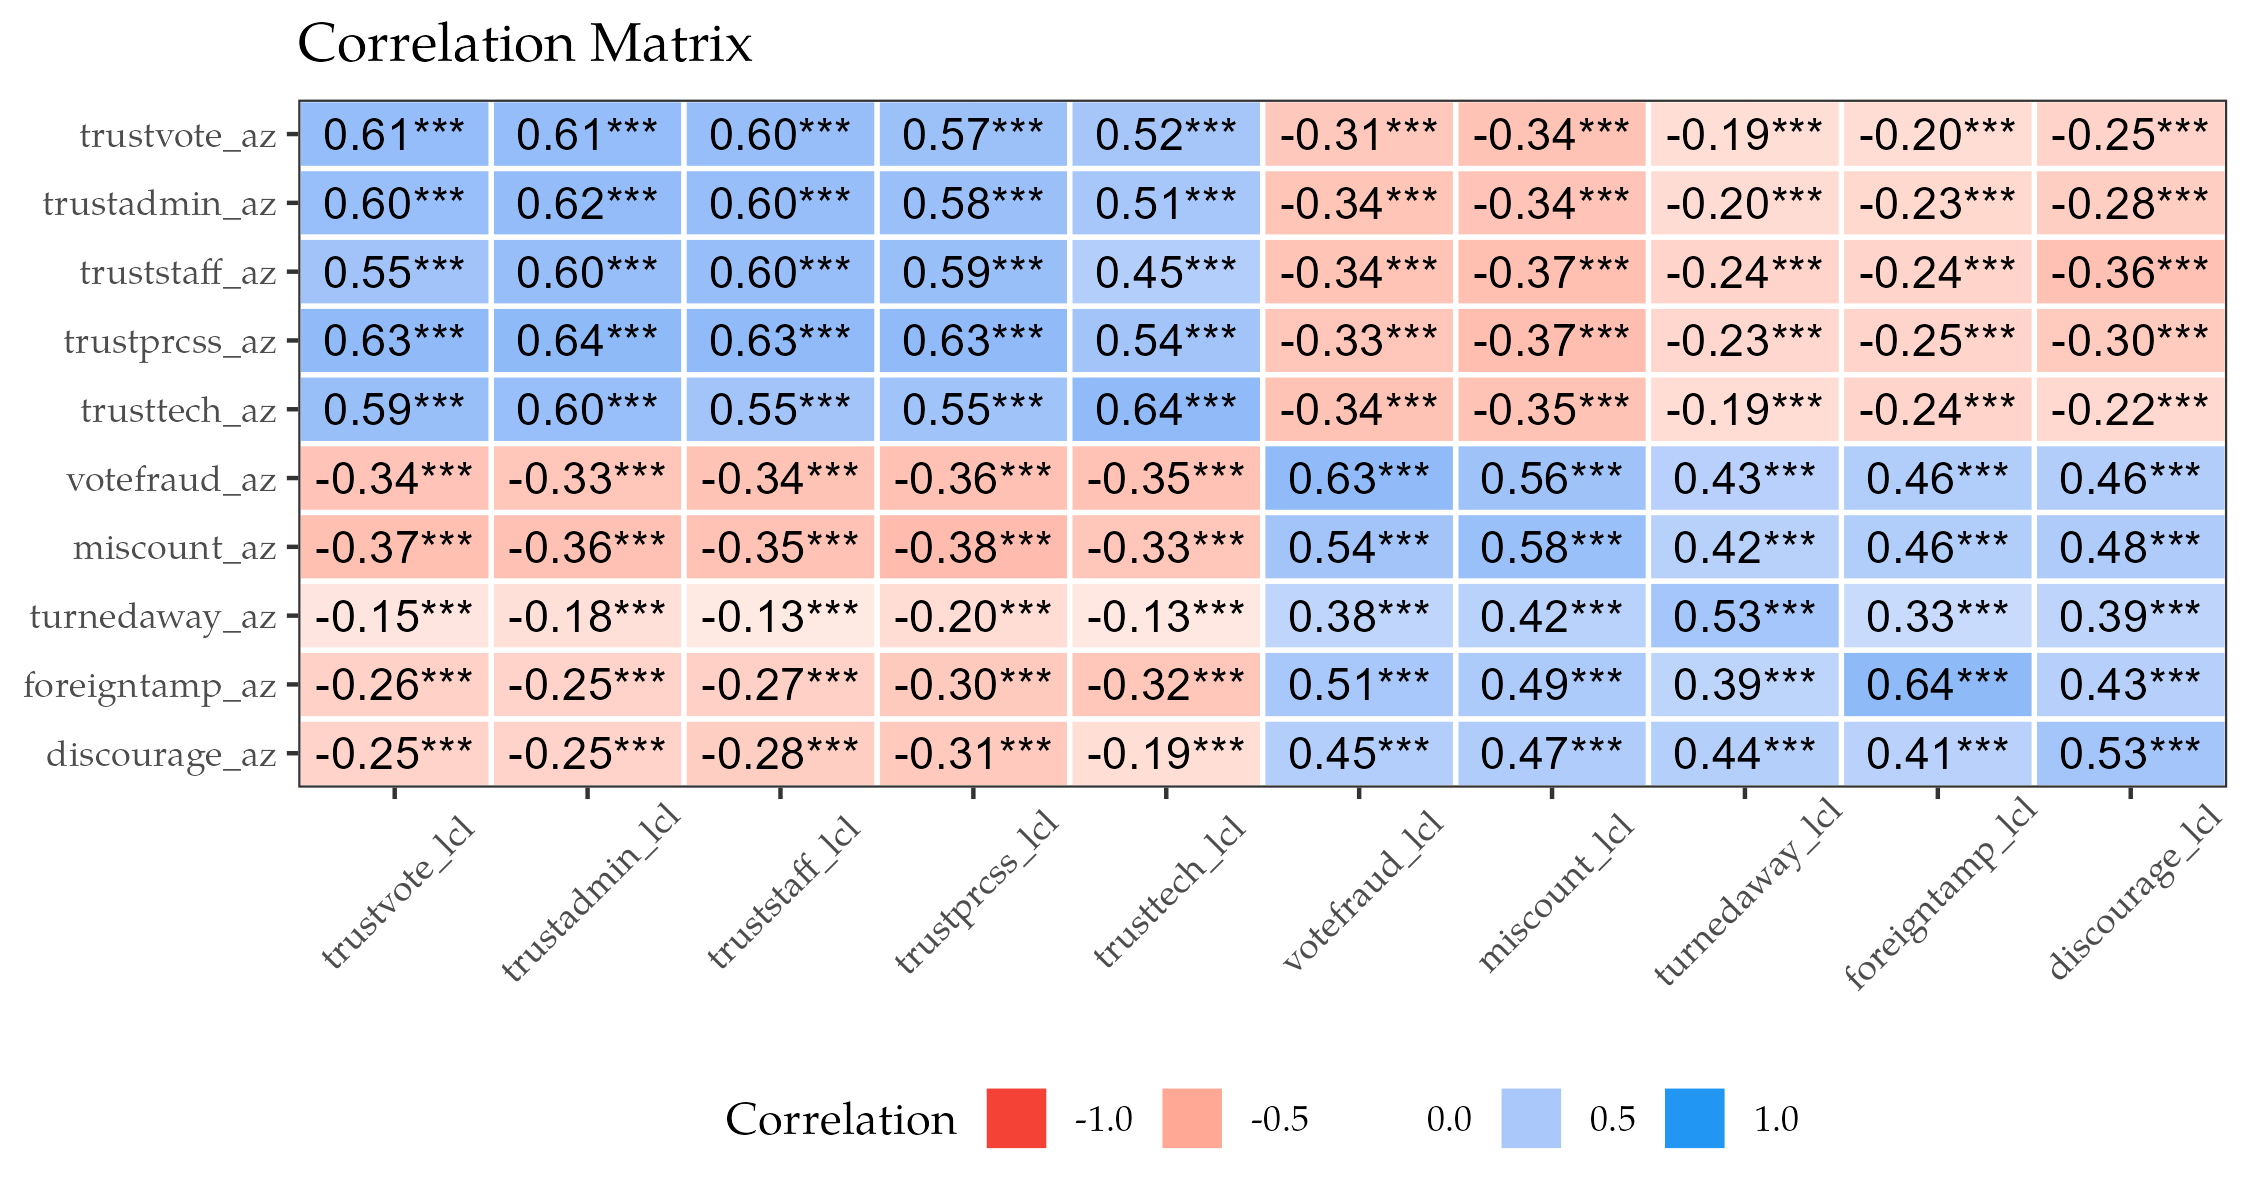
\includegraphics[keepaspectratio]{index_files/figure-pdf/fig-polycor-1.png}}

}

\end{figure}%

Indeed, this is what is revealed by the correlation matrix
(Figure~\ref{fig-polycor}). Trust items correlate positively, strongly,
and are significant regardless of location at which the items pertain.
The same goes for distrust items. Also, items meant to measure trust
negatively correlate with the items that measure distrust. However, the
positive correlations are not nearly as high as would be expected
supposing that the items are nearly identical theoretical indicators of
the same hypothetical constructs, i.e., trust and distrust respectively.

If the items accurately measure trust/distrust in elections regardless
of where those elections are said to take place, then positive
correlations between the AZ and Local area items should approach perfect
correlation as though the same exact questions were asked twice. This
result, however, suggests that the location of which the survey items
pertain (and perhaps other factors) makes a substantial difference in
the pattern of responses, but also raises valid questions as to whether
the items accurately measure the latent variable constructs in the first
place.

Although I do not explicitly assume that the survey instruments
perfectly measure the hypothetical constructs of interest (i.e., trust
and distrust), perfect measurement is implicitly assumed by the method
of combining multiple item responses into a sum or mean composite score.

In short, I expected item responses from the trust and distrust scales
to be inversely correlated among the sample, but not mutually exclusive.
Indeed, this is what I find. Polychoric correlations between the trust
and distrust items negatively correlate as expected, as does the
correlation between the two sum score scales. Given the ordinal nature
of the variable items, I conducted a Spearman's rank correlation test
(\citeproc{ref-spearman1907}{Spearman 1907}) and found a negative
correlation of \(\rho = -0.49\) (\(95\%\) CI {[}-0.53, -0.44{]};
Kendall's \(\tau = -0.39\)) between scores on the two scales for the AZ
items (For the local item scale score correlation: \(\rho = -0.52\),
\(95\%\) CI {[}-0.56, -0.48{]}; Kendall's \(\tau = -0.39\)). The
negative correlation between the trust and distrust items and scores
makes intuitive sense.

\newpage{}

\section{Appendix E: Predicted Probabilities of Safety Concerns by
Treatment
Condition}\label{appendix-e-predicted-probabilities-of-safety-concerns-by-treatment-condition}

\begin{table}[H]

\caption{\label{tbl-safety-logit}Ordinal Logistic Regression of Concerns
for Violence and Confidence in Voter Safety Regressed on Experiment
Condition}

\centering{

\centering
\begin{talltblr}[         %% tabularray outer open
entry=none,label=none,
note{}={{\fontsize{0.75em}{0.75em}\selectfont + p < 0.1, * p < 0.05, ** p < 0.01, *** p < 0.001}},
note{ }={{\fontsize{0.75em}{0.75em}\selectfont Parameter estimate (and confidence intervals) exponentiated to show odds ratios.}},
note{  }={{\fontsize{0.75em}{0.75em}\selectfont Uncertainty intervals (profile-likelihood) and p-values (two-tailed) computed using a Wald t-distribution approximation}},
]                     %% tabularray outer close
{                     %% tabularray inner open
colspec={Q[]Q[]Q[]},
column{2,3}={}{halign=c, font=\fontsize{0.8em}{1.1em}\selectfont,},
column{1}={}{halign=l, font=\fontsize{0.8em}{1.1em}\selectfont,},
hline{16}={1,2,3}{solid, black, 0.05em},
}                     %% tabularray inner close
\toprule
& Concerns for Violence (OR) & Confidence in Voter Safety (OR) \\ \midrule %% TinyTableHeader
Treatment & 1.289* & 1.494*** \\
& [1.055, 1.576] & [1.211, 1.844] \\
Very concerned | Somewhat concerned & 0.153*** &  \\
& [0.127, 0.186] &  \\
Somewhat concerned | Not too concerned & 1.125 &  \\
& [0.969, 1.305] &  \\
Not too concerned | Not at all concerned & 6.762*** &  \\
& [5.595, 8.171] &  \\
Not at all confident | Not too confident &  & 0.055*** \\
&  & [0.041, 0.073] \\
Not too confident | Somewhat confident &  & 0.280*** \\
&  & [0.237, 0.332] \\
Somewhat confident | Very confident &  & 3.150*** \\
&  & [2.667, 3.721] \\
Num.Obs. & 1286 & 1285 \\
RMSE & 2.44 & 2.91 \\
\bottomrule
\end{talltblr}

}

\end{table}%

\begin{table}[H]

\caption{\label{tbl-safety-preds1}Unit-level predicted probabilities of
selecting response or higher comparing experiment condition}

\centering{

\centering
\begin{talltblr}[         %% tabularray outer open
entry=none,label=none,
note{}={{\fontsize{0.75em}{0.75em}\selectfont Thinking about Maricopa County, AZ, how concerned should voters feel about potential violence, threats of violence, or intimidation while voting in person at their local polling place?}},
]                     %% tabularray outer close
{                     %% tabularray inner open
colspec={Q[]Q[]Q[]Q[]Q[]Q[]Q[]},
column{3,4,5,6,7}={}{font=\fontsize{0.8em}{1.1em}\selectfont, halign=c,},
column{1,2}={}{font=\fontsize{0.8em}{1.1em}\selectfont, halign=l,},
}                     %% tabularray inner close
\toprule
Violence & Condition & estimate & std.error & z & Pr(>|z|) & conf.int \\ \midrule %% TinyTableHeader
Very concerned & Control & 0.133 & 0.011 & 11.746 & 7.442e-32 & [0.111, 0.155] \\
Very concerned & Treatment & 0.106 & 0.010 & 10.977 & 4.955e-28 & [0.087, 0.125] \\
Somewhat concerned & Control & 0.396 & 0.016 & 25.430 & 1.175e-142 & [0.366, 0.427] \\
Somewhat concerned & Treatment & 0.360 & 0.015 & 23.556 & 1.081e-122 & [0.330, 0.389] \\
Not too concerned & Control & 0.342 & 0.015 & 23.296 & 4.890e-120 & [0.313, 0.371] \\
Not too concerned & Treatment & 0.374 & 0.015 & 24.825 & 4.779e-136 & [0.344, 0.403] \\
Not at all concerned & Control & 0.129 & 0.011 & 11.895 & 1.263e-32 & [0.108, 0.150] \\
Not at all concerned & Treatment & 0.160 & 0.012 & 12.882 & 5.678e-38 & [0.136, 0.185] \\
\bottomrule
\end{talltblr}

}

\end{table}%

\begin{table}[H]

\caption{\label{tbl-safety-preds2}Unit-level predicted probabilities of
selecting response or higher conditional to the Treatment experiment
condition}

\centering{

\centering
\begin{talltblr}[         %% tabularray outer open
entry=none,label=none,
note{}={{\fontsize{0.75em}{0.75em}\selectfont How confident, if at all, are you that in person polling places in Maricopa County, AZ will be safe places for voters to cast their ballots during the upcoming elections in November?}},
]                     %% tabularray outer close
{                     %% tabularray inner open
colspec={Q[]Q[]Q[]Q[]Q[]Q[]Q[]},
column{3,4,5,6,7}={}{font=\fontsize{0.8em}{1.1em}\selectfont, halign=c,},
column{1,2}={}{font=\fontsize{0.8em}{1.1em}\selectfont, halign=l,},
}                     %% tabularray inner close
\toprule
Voter Safety & Condition & estimate & std.error & z & Pr(>|z|) & conf.int \\ \midrule %% TinyTableHeader
Not at all confident & Control & 0.052 & 0.007 & 7.302 & 2.845e-13 & [0.038, 0.066] \\
Not at all confident & Treatment & 0.035 & 0.005 & 6.932 & 4.141e-12 & [0.025, 0.045] \\
Not too confident & Control & 0.167 & 0.013 & 13.268 & 3.563e-40 & [0.142, 0.192] \\
Not too confident & Treatment & 0.123 & 0.010 & 11.924 & 8.875e-33 & [0.102, 0.143] \\
Somewhat confident & Control & 0.540 & 0.014 & 38.037 & 0.000 & [0.512, 0.568] \\
Somewhat confident & Treatment & 0.520 & 0.014 & 36.134 & 6.715e-286 & [0.492, 0.549] \\
Very confident & Control & 0.241 & 0.016 & 15.519 & 2.583e-54 & [0.211, 0.271] \\
Very confident & Treatment & 0.322 & 0.017 & 18.550 & 8.104e-77 & [0.288, 0.356] \\
\bottomrule
\end{talltblr}

}

\end{table}%

\newpage{}

\section*{References}\label{bibliography}
\addcontentsline{toc}{section}{References}

\phantomsection\label{refs}
\begin{CSLReferences}{1}{1}
\bibitem[\citeproctext]{ref-abbate2020a}
Abbate, Andrea. 2020. {``39 {Ways Election Offices} Are {Responding} to
{COVID-19}.''}
\url{https://www.techandciviclife.org/covid-19-responses/}.

\bibitem[\citeproctext]{ref-anderson2006}
Anderson, Benedict. 2006. \emph{Imagined Communities : Reflections on
the Origin and Spread of Nationalism}. Revised edition. London ; Verso.

\bibitem[\citeproctext]{ref-atkeson2007}
Atkeson, Lonna Rae, and Kyle L. Saunders. 2007. {``The {Effect} of
{Election Administration} on {Voter Confidence}: {A Local Matter}?''}
\emph{PS: Political Science \& Politics} 40(4): 655--60.
doi:\href{https://doi.org/10.1017/S1049096507071041}{10.1017/S1049096507071041}.

\bibitem[\citeproctext]{ref-baldor2025c}
Baldor, Lolita. 2025a. {``Military Commanders Will Be Told to Send
Transgender Troops to Medical Checks to Oust Them.''}
\url{https://apnews.com/article/transgender-ban-military-discharge-troops-0218f0b6fec595c420bd0ac072d87335}.

\bibitem[\citeproctext]{ref-baldor2025a}
Baldor, Lolita. 2025b. {``Military Parade to Celebrate the {Army}'s
250th Anniversary Will Be Held on {Trump}'s Birthday.''}
\url{https://apnews.com/article/trump-army-military-parade-birthday-2f5cd12c8ccd4efddc29bfa3cf8f2705}.

\bibitem[\citeproctext]{ref-baldor2025b}
Baldor, Lolita. 2025c. {``Pentagon Directs Military to Pull Library
Books That Address Diversity, Anti-Racism, Gender Issues.''}
\url{https://apnews.com/article/pentagon-hegseth-dei-library-books-770364ab99591402ddffe8758432ff26}.

\bibitem[\citeproctext]{ref-baldor2020}
Baldor, Lolita C. 2020. {``Military Wary That Shakeup Could Upend Its
Apolitical Nature.''}
\url{https://apnews.com/article/military-wary-shakeup-upend-apolitical-89eccf0aef7cf7b99208b3bfd0453a43}.

\bibitem[\citeproctext]{ref-baldor2025}
Baldor, Lolita C. 2025. {``Hegseth Orders the Name of Gay Rights
Activist {Harvey Milk} Scrubbed from {Navy} Ship.''}
\url{https://apnews.com/article/harvey-milk-navy-ship-renamed-pride-month-d6cda5df15ee5bc066092d54c591c6f2}.

\bibitem[\citeproctext]{ref-betros2001}
Betros, Lance. 2001. {``Political {Partisanship} and the {Military
Ethic} in {America}.''} \emph{Armed Forces \& Society} 27(4): 501--23.
doi:\href{https://doi.org/10.1177/0095327X0102700401}{10.1177/0095327X0102700401}.

\bibitem[\citeproctext]{ref-bowler2024}
Bowler, Shaun, and Todd Donovan. 2024. {``Confidence in {US Elections
After} the {Big Lie}.''} \emph{Political Research Quarterly} 77(1):
283--96.
doi:\href{https://doi.org/10.1177/10659129231206179}{10.1177/10659129231206179}.

\bibitem[\citeproctext]{ref-brennancenterforjustice2024}
Brennan Center for Justice. 2024. \emph{Local {Election Officials
Survey} --- {May} 2024 \textbar{} {Brennan Center} for {Justice}}.
Brennan Center Research Department.
\url{https://www.brennancenter.org/our-work/research-reports/local-election-officials-survey-may-2024}
(November 5, 2024).

\bibitem[\citeproctext]{ref-butz2009}
Butz, David A. 2009. {``National {Symbols} as {Agents} of
{Psychological} and {Social Change}.''} \emph{Political Psychology}
30(5): 779--804.
doi:\href{https://doi.org/10.1111/j.1467-9221.2009.00725.x}{10.1111/j.1467-9221.2009.00725.x}.

\bibitem[\citeproctext]{ref-butz2007}
Butz, David A., E. Ashby Plant, and Celeste E. Doerr. 2007. {``Liberty
and {Justice} for {All}? {Implications} of {Exposure} to the {U}.{S}.
{Flag} for {Intergroup Relations}.''} \emph{Personality and Social
Psychology Bulletin} 33(3): 396--408.
doi:\href{https://doi.org/10.1177/0146167206296299}{10.1177/0146167206296299}.

\bibitem[\citeproctext]{ref-carter2024}
Carter, Luke, Ashlan Gruwell, J Quin Monson, and Kelly D Patterson.
2024. {``From {Confidence} to {Convenience}: {Changes} in {Voting
Systems}, {Donald Trump}, and {Voter Confidence}.''} \emph{Public
Opinion Quarterly} 88: 516--35.
doi:\href{https://doi.org/10.1093/poq/nfae034}{10.1093/poq/nfae034}.

\bibitem[\citeproctext]{ref-cikara2014}
Cikara, Mina, and Jay J Van Bavel. 2014. {``The {Neuroscience} of
{Intergroup Relations}.''} \emph{Perspectives on Psychological Science}
9(3): 245--74.

\bibitem[\citeproctext]{ref-claassen2008}
Claassen, Ryan L., David B. Magleby, J. Quin Monson, and Kelly D.
Patterson. 2008. {``{`{At Your Service}'}: {Voter Evaluations} of {Poll
Worker Performance}.''} \emph{American Politics Research} 36(4):
612--34.
doi:\href{https://doi.org/10.1177/1532673X08319006}{10.1177/1532673X08319006}.

\bibitem[\citeproctext]{ref-clayton2023}
Clayton, Katherine, and Robb Willer. 2023. {``Endorsements from
{Republican} Politicians Can Increase Confidence in {U}.{S}.
Elections.''} \emph{Research \& Politics} 10(1): 20531680221148967.
doi:\href{https://doi.org/10.1177/20531680221148967}{10.1177/20531680221148967}.

\bibitem[\citeproctext]{ref-coll2024a}
Coll, Joseph A, and Christopher J Clark. 2024. {``A {Racial Model} of
{Electoral Reform}: {The Relationship} Between {Restrictive Voting
Policies} and {Voter Confidence} for {Black} and {White Voters}.''}
\emph{Public Opinion Quarterly} 88: 561--84.
doi:\href{https://doi.org/10.1093/poq/nfae032}{10.1093/poq/nfae032}.

\bibitem[\citeproctext]{ref-conde2020}
Conde, Ximena. 2020. {``Philly Area Counties Say Efforts to Recruit Poll
Workers for {Election Day} Are Paying Off.''} \emph{WHYY NPR}.
\url{https://whyy.org/articles/philly-area-counties-say-efforts-to-recruit-poll-workers-for-election-day-are-paying-off/}.

\bibitem[\citeproctext]{ref-cook2005}
Cook, Timothy E., and Paul Gronke. 2005. {``The {Skeptical American}:
{Revisiting} the {Meanings} of {Trust} in {Government} and {Confidence}
in {Institutions}.''} \emph{The Journal of Politics} 67(3): 784--803.
doi:\href{https://doi.org/10.1111/j.1468-2508.2005.00339.x}{10.1111/j.1468-2508.2005.00339.x}.

\bibitem[\citeproctext]{ref-cooter2013}
Cooter, Amy. 2013. {``Americanness, {Masculinity}, and {Whiteness}: {How
Michigan Militia Men Navigate Evolving Social Norms}.''} Thesis.
\url{http://deepblue.lib.umich.edu/handle/2027.42/98077}.

\bibitem[\citeproctext]{ref-cooter2024}
Cooter, Amy. 2024. {``Veterans and {Extremism}: {From Militias} to
{January} 6th and {Real Patriots} \textbar{} {Middlebury Institute} of
{International Studies} at {Monterey}.''}
\url{https://www.middlebury.edu/institute/academics/centers-initiatives/ctec/ctec-publications/veterans-and-extremism-militias-january-6th}.

\bibitem[\citeproctext]{ref-corrigan2002}
Corrigan, Patrick W., David Rowan, Amy Green, Robert Lundin, Philip
River, Kyle Uphoff-Wasowski, Kurt White, and Mary Anne Kubiak. 2002.
{``Challenging {Two Mental Illness Stigmas}: {Personal Responsibility}
and {Dangerousness}.''} \emph{Schizophrenia Bulletin} 28(2): 293--309.
doi:\href{https://doi.org/10.1093/oxfordjournals.schbul.a006939}{10.1093/oxfordjournals.schbul.a006939}.

\bibitem[\citeproctext]{ref-daniller2019}
Daniller, Andrew M, and Diana C Mutz. 2019. {``The {Dynamics} of
{Electoral Integrity}: {A Three-Election Panel Study}.''} \emph{Public
Opinion Quarterly} 83(1): 46--67.
doi:\href{https://doi.org/10.1093/poq/nfz002}{10.1093/poq/nfz002}.

\bibitem[\citeproctext]{ref-doubek2024}
Doubek, James. 2024. {``States and Cities Beef up Security to Prepare
for Potential Election-Related Violence.''} \emph{NPR: 2024 Election}.
\url{https://www.npr.org/2024/11/04/nx-s1-5178083/national-guard-police-election-security}
(November 5, 2024).

\bibitem[\citeproctext]{ref-dunn2018}
Dunn, Amina. 2018. {``Elections in {America}: {Concerns Over Security},
{Divisions Over Expanding Access} to {Voting}.''}
\url{https://www.pewresearch.org/politics/2018/10/29/elections-in-america-concerns-over-security-divisions-over-expanding-access-to-voting/}.

\bibitem[\citeproctext]{ref-edlin2024}
Edlin, Ruby, and Lawrence Norden. 2024. {``Poll of {Election Officials
Finds Concerns About Safety}, {Political Interference} \textbar{}
{Brennan Center} for {Justice}.''}
\url{https://www.brennancenter.org/our-work/analysis-opinion/poll-election-officials-finds-concerns-about-safety-political}.

\bibitem[\citeproctext]{ref-ferrer2024}
Ferrer, Joshua, Daniel M Thompson, and Rachel Orey. 2024. \emph{Election
{Official Turnover Rates} from 2000--2024}. Bipartisan Policy Center.
\url{https://bipartisanpolicy.org/download/?file=/wp-content/uploads/2024/04/WEB_BPC_Elections_Admin_Turnover_R01.pdf}.

\bibitem[\citeproctext]{ref-gangl2016}
Gangl, Katharina, Benno Torgler, and Erich Kirchler. 2016.
{``Patriotism's {Impact} on {Cooperation} with the {State}: {An
Experimental Study} on {Tax Compliance}.''} \emph{Political Psychology}
37(6): 867--81.
doi:\href{https://doi.org/10.1111/pops.12294}{10.1111/pops.12294}.

\bibitem[\citeproctext]{ref-garamone2016a}
Garamone, Jim. 2016a. {``Active-{Duty Personnel Must Remain Apolitical},
{Nonpartisan}, {Dunford Says}.''}
\url{https://www.defense.gov/News/News-Stories/Article/Article/881624/active-duty-personnel-must-remain-apolitical-nonpartisan-dunford-says}.

\bibitem[\citeproctext]{ref-garamone2016}
Garamone, Jim. 2016b. {``{DOD} Civilians, Service Members Must Remain
Non-Partisan, Apolitical.''}
\url{https://www.defense.gov/News/Releases/Release/Article/975910/dod-civilians-service-members-must-remain-non-partisan-apolitical}.

\bibitem[\citeproctext]{ref-gaudette2025}
Gaudette, Jennifer, Seth J. Hill, Thad Kousser, Mackenzie Lockhart, and
Mindy Romero. 2025. {``Can {Official Messaging} on {Trust} in {Elections
Break Through Partisan Polarization}?''} \emph{British Journal of
Political Science} 55: e16.
doi:\href{https://doi.org/10.1017/S0007123424000681}{10.1017/S0007123424000681}.

\bibitem[\citeproctext]{ref-giles2021}
Giles, Ben. 2021. {``Arizona {Recount Of} 2020 {Election Ballots Found
No Proof Of Corruption}.''} \emph{NPR: 2024 Election}.
\url{https://www.npr.org/2021/09/25/1040672550/az-audit}.

\bibitem[\citeproctext]{ref-hall2009}
Hall, Thad E., J. Quin Monson, and Kelly D. Patterson. 2009. {``The
{Human Dimension} of {Elections}: {How Poll Workers Shape Public
Confidence} in {Elections}.''} \emph{Political Research Quarterly}
62(3): 507--22.
doi:\href{https://doi.org/10.1177/1065912908324870}{10.1177/1065912908324870}.

\bibitem[\citeproctext]{ref-hall2007}
Hall, Thad, J. Quin Monson, and Kelly D. Patterson. 2007. {``Poll
{Workers} and the {Vitality} of {Democracy}: {An Early Assessment}.''}
\emph{PS: Political Science \& Politics} 40(4): 647--54.
doi:\href{https://doi.org/10.1017/S104909650707103X}{10.1017/S104909650707103X}.

\bibitem[\citeproctext]{ref-hardy2019}
Hardy, Molly M., Calvin R. Coker, Michelle E. Funk, and Benjamin R.
Warner. 2019. {``Which Ingroup, When? {Effects} of Gender, Partisanship,
Veteran Status, and Evaluator Identities on Candidate Evaluations.''}
\emph{Communication Quarterly} 67(2): 199--220.
doi:\href{https://doi.org/10.1080/01463373.2019.1573201}{10.1080/01463373.2019.1573201}.

\bibitem[\citeproctext]{ref-herndon2020}
Herndon, Astead W. 2020. {``{LeBron James} and a {Multimillion-Dollar
Push} for {More Poll Workers}.''} \emph{The New York Times: U.S.}
\url{https://www.nytimes.com/2020/08/24/us/politics/lebron-james-poll-workers.html}
(November 13, 2024).

\bibitem[\citeproctext]{ref-herrnson2009}
Herrnson, Paul S., Richard G. Niemi, and Michael J. Hanmer. 2009.
\emph{Voting Technology : The Not-so-Simple Act of Casting a Ballot}.
Washington, D.C: Brookings Institution Press.

\bibitem[\citeproctext]{ref-hipes2016}
Hipes, Crosby, Jeffrey Lucas, Jo C. Phelan, and Richard C. White. 2016.
{``The Stigma of Mental Illness in the Labor Market.''} \emph{Social
Science Research} 56: 16--25.
doi:\href{https://doi.org/10.1016/j.ssresearch.2015.12.001}{10.1016/j.ssresearch.2015.12.001}.

\bibitem[\citeproctext]{ref-hooghe2018}
Hooghe, Marc. 2018. {``Trust and {Elections}.''} In \emph{The {Oxford
Handbook} of {Social} and {Political Trust}}, ed. Eric M. Uslaner.
Oxford University Press, 0.
doi:\href{https://doi.org/10.1093/oxfordhb/9780190274801.013.17}{10.1093/oxfordhb/9780190274801.013.17}.

\bibitem[\citeproctext]{ref-jensen2022a}
Jensen, Michael, Elizabeth Yates, and Sheehan Kane. 2022.
\emph{Radicalization in the {Ranks}: {An Assessment} of the {Scope} and
{Nature} of {Criminal Extremism} in the {United States Military}}.
{National Consortium for the Study of Terrorism and Responses to
Terrorism (START): College Park}.
\url{https://www.start.umd.edu/pubs/Radicalization\%20in\%20the\%20Ranks_April\%202022.pdf}.

\bibitem[\citeproctext]{ref-kalmoe2016}
Kalmoe, Nathan P., and Kimberly Gross. 2016. {``Cueing {Patriotism},
{Prejudice}, and {Partisanship} in the {Age} of {Obama}: {Experimental
Tests} of {U}.{S}. {Flag Imagery Effects} in {Presidential Elections}:
{Flag Imagery Effects} in {Presidential Elections}.''} \emph{Political
Psychology} 37(6): 883--99.
doi:\href{https://doi.org/10.1111/pops.12305}{10.1111/pops.12305}.

\bibitem[\citeproctext]{ref-kemmelmeier2008}
Kemmelmeier, Markus, and David G. Winter. 2008. {``Sowing {Patriotism},
{But Reaping Nationalism}? {Consequences} of {Exposure} to the {American
Flag}: {Exposure} to the {American Flag}.''} \emph{Political Psychology}
29(6): 859--79.
doi:\href{https://doi.org/10.1111/j.1467-9221.2008.00670.x}{10.1111/j.1467-9221.2008.00670.x}.

\bibitem[\citeproctext]{ref-kleykamp2015}
Kleykamp, Meredith, and Crosby Hipes. 2015. {``Coverage of {Veterans} of
the {Wars} in {Iraq} and {Afghanistan} in the {U}.{S}. {Media}.''}
\emph{Sociological Forum} 30(2): 348--68.
doi:\href{https://doi.org/10.1111/socf.12166}{10.1111/socf.12166}.

\bibitem[\citeproctext]{ref-kleykamp2018}
Kleykamp, Meredith, Crosby Hipes, and Alair MacLean. 2018. {``Who
{Supports U}.{S}. {Veterans} and {Who Exaggerates Their Support}?''}
\emph{Armed Forces \& Society} 44(1): 92--115.
doi:\href{https://doi.org/10.1177/0095327X16682786}{10.1177/0095327X16682786}.

\bibitem[\citeproctext]{ref-kleykamp2023}
Kleykamp, Meredith, Daniel Schwam, and Gilad Wenig. 2023. \emph{What
{Americans Think About Veterans} and {Military Service}: {Findings} from
a {Nationally Representative Survey}}. RAND Corporation.
\url{https://www.rand.org/pubs/research_reports/RRA1363-7.html}.

\bibitem[\citeproctext]{ref-krupnikov2022}
Krupnikov, Yanna, and John Barry Ryan. 2022. \emph{The Other Divide:
Polarization and Disengagement in {American} Politics}. Cambridge,
United Kingdom ; Cambridge University Press.

\bibitem[\citeproctext]{ref-lagrone2019}
LaGrone, Sam. 2019. {``Shanahan {Reminds Pentagon} to {Stay
Apolitical}.''}
\url{https://news.usni.org/2019/06/11/acting-secdef-shanahan-reminds-pentagon-to-stay-apolitical-following-mccain-situation}.

\bibitem[\citeproctext]{ref-lawrence2022}
Lawrence, Quil. 2022. {``Vetting the {Vote}: {Military} Veterans
Volunteer as Impartial Poll Workers.''} \emph{NPR: National}.
\url{https://www.npr.org/2022/11/04/1133920940/vetting-the-vote-military-veterans-volunteer-as-impartial-poll-workers}.

\bibitem[\citeproctext]{ref-lawrence2024}
Lawrence, Quil. 2024. {``As Fears about Election Security Grow, Military
Veterans Are Filling as Poll Workers.''}
\url{https://www.npr.org/2024/10/14/nx-s1-5144186/as-fears-about-election-security-grow-military-veterans-are-filling-as-poll-workers}.

\bibitem[\citeproctext]{ref-levendusky2018}
Levendusky, Matthew S. 2018. {``Americans, {Not Partisans}: {Can Priming
American National Identity Reduce Affective Polarization}?''} \emph{The
Journal of Politics} 80(1): 59--70.
\url{https://www.jstor.org/stable/26551118} (June 4, 2025).

\bibitem[\citeproctext]{ref-levendusky2024}
Levendusky, Matthew, Shawn Patterson Jr., Michele Margolis, Yotam Ophir,
Dror Walter, and Kathleen Hall Jamieson. 2024. {``The {Long Shadow} of
the {Big Lie}: {How Beliefs} about the {Legitimacy} of the 2020
{Election Spill Over} onto {Future Elections}.''} \emph{Public Opinion
Quarterly}: nfae047.
doi:\href{https://doi.org/10.1093/poq/nfae047}{10.1093/poq/nfae047}.

\bibitem[\citeproctext]{ref-lincoln2024}
Lincoln, Sophie. 2024. {``Washoe {County} Staff Prepare for {Election
Day}, Announce New Safety Feature at Polls.''}
\url{https://mynews4.com/news/local/washoe-county-staff-prepare-for-election-day-announce-new-safety-feature-at-polls}
(November 5, 2024).

\bibitem[\citeproctext]{ref-loewenson2023}
Loewenson, Irene. 2023. {``Mattis Says Vets at {Jan}. 6 {Capitol} Riot
{`Don't Define the Military'}.''} \emph{Marine Corps Times: name}.
\url{https://www.marinecorpstimes.com/news/your-marine-corps/2023/11/06/mattis-says-vets-at-jan-6-capitol-riot-dont-define-the-military/}.

\bibitem[\citeproctext]{ref-looker2024}
Looker, Rachel. 2024. {``How Some Veterans Find a Way to 'Serve the
Country Again' on {Super Tuesday}.''}
\url{https://www.usatoday.com/story/news/politics/elections/2024/03/05/veterans-poll-workers-election/72839163007/}.

\bibitem[\citeproctext]{ref-maclean2014}
MacLean, Alair, and Meredith Kleykamp. 2014. {``Coming {Home}:
{Attitudes} Toward {U}.{S}. {Veterans Returning} from {Iraq}.''}
\emph{Social Problems} 61(1): 131--54.
doi:\href{https://doi.org/10.1525/sp.2013.12074}{10.1525/sp.2013.12074}.

\bibitem[\citeproctext]{ref-magni2024}
Magni, Gabriele, and Andrew Reynolds. 2024. {``Candidate {Identity} and
{Campaign Priming}: {Analyzing Voter Support} for {Pete Buttigieg}'s
{Presidential Run} as an {Openly Gay Man}.''} \emph{Political Research
Quarterly} 77(1): 184--98.
doi:\href{https://doi.org/10.1177/10659129231194325}{10.1177/10659129231194325}.

\bibitem[\citeproctext]{ref-maidenberg1996}
Maidenberg, David H. 1996. \emph{Recruiting {Poll Workers}}. Office of
Election Administration, Federal Election Commission.
\url{https://purl.fdlp.gov/GPO/gpo18585}.

\bibitem[\citeproctext]{ref-maricopacountyelectionsdepartment2022}
Maricopa County Elections Department. 2022. \emph{Correcting the
{Record}: {Maricopa County}'s {In-Depth Analysis} of the {Senate
Inquiry}}. Maricopa County, Arizona: {Maricopa County Elections
Department and Office of the Recorder}.
\url{https://elections.maricopa.gov/asset/jcr:a9e03750-0a8f-4162-859f-1d46ac54b485/Correcting\%20The\%20Record\%20-\%20January\%202022\%20Report.pdf}.

\bibitem[\citeproctext]{ref-mcdermott2015}
McDermott, Monika L., and Costas Panagopoulos. 2015. {``Be {All} That
{You Can Be}: {The Electoral Impact} of {Military Service} as an
{Information Cue}.''} \emph{Political Research Quarterly} 68(2):
293--305.
doi:\href{https://doi.org/10.1177/1065912915572151}{10.1177/1065912915572151}.

\bibitem[\citeproctext]{ref-mcneish2023}
McNeish, Daniel. 2023. {``Psychometric Properties of Sum Scores and
Factor Scores Differ Even When Their Correlation Is 0.98: {A} Response
to {Widaman} and {Revelle}.''} \emph{Behavior Research Methods} 55(8):
4269--90.
doi:\href{https://doi.org/10.3758/s13428-022-02016-x}{10.3758/s13428-022-02016-x}.

\bibitem[\citeproctext]{ref-mcneish2020}
McNeish, Daniel, and Melissa Gordon Wolf. 2020. {``Thinking Twice about
Sum Scores.''} \emph{Behavior Research Methods} 52(6): 2287--2305.
doi:\href{https://doi.org/10.3758/s13428-020-01398-0}{10.3758/s13428-020-01398-0}.

\bibitem[\citeproctext]{ref-mcnerney2006}
Mcnerney, Michael. 2006. {``Military {Partisanship}.''} \emph{Journal of
Political \& Military Sociology} 34(2): 281--88.
\url{https://www.jstor.org/stable/45294228} (June 4, 2025).

\bibitem[\citeproctext]{ref-mena2020}
Mena, Kelly. 2020. {``States Scramble to Recruit Thousands of Poll
Workers Amid Pandemic Shortage \textbar{} {CNN Politics}.''}
\url{https://www.cnn.com/2020/08/13/politics/poll-worker-shortage-2020-election/index.html}.

\bibitem[\citeproctext]{ref-milton2021}
Milton, Daniel, and Andrew Mines. 2021. \emph{{``{This} Is {War}:''}
{Examining Military Experience Among} the {Capitol Hill Siege
Participants}}. George Washington University.
doi:\href{https://doi.org/10.4079/poe.04.2021.00}{10.4079/poe.04.2021.00}.

\bibitem[\citeproctext]{ref-mullinix2022}
Mullinix, Kevin J., and Trent Lythgoe. 2022. {``Priming {Norms} to
{Combat Affective Polarization}.''} \emph{Political Research Quarterly}:
106591292110733.
doi:\href{https://doi.org/10.1177/10659129211073319}{10.1177/10659129211073319}.

\bibitem[\citeproctext]{ref-nadeau1993}
Nadeau, Richard, and André Blais. 1993. {``Accepting the {Election
Outcome}: {The Effect} of {Participation} on {Losers}' {Consent}.''}
\emph{British Journal of Political Science} 23(4): 553--63.
doi:\href{https://doi.org/10.1017/S0007123400006736}{10.1017/S0007123400006736}.

\bibitem[\citeproctext]{ref-nadeem2024}
Nadeem, Reem. 2024. {``Harris, {Trump Voters Differ Over Election
Security}, {Vote Counts} and {Hacking Concerns}.''}
\url{https://www.pewresearch.org/politics/2024/10/24/harris-trump-voters-differ-over-election-security-vote-counts-and-hacking-concerns/}
(November 5, 2024).

\bibitem[\citeproctext]{ref-nesbit2011}
Nesbit, Rebecca, and David A. Reingold. 2011. {``Soldiers to {Citizens}:
{The Link} Between {Military Service} and {Volunteering}.''}
\emph{Public Administration Review} 71(1): 67--76.
doi:\href{https://doi.org/10.1111/j.1540-6210.2010.02307.x}{10.1111/j.1540-6210.2010.02307.x}.

\bibitem[\citeproctext]{ref-nevadasecretaryofstate2023}
Nevada Secretary of State. 2023. {``Governor {Joe Lombardo}, {Secretary}
of {State Francisco V}. {Aguilar} Sign {Election Worker Protection Bill}
into Law.''}
\url{https://www.nvsos.gov/sos/Home/Components/News/News/3368/309?backlist=\%2Fsos}
(November 5, 2024).

\bibitem[\citeproctext]{ref-nflfootballoperations2022}
NFL Football Operations. 2022. {``Vet the {Vote}.''}
\url{https://operations.nfl.com/inside-football-ops/social-justice/vet-the-vote/}.

\bibitem[\citeproctext]{ref-nichols2015}
Nichols, Curt. 2015. {``Public {Opinion} and the {Military}: {A
Multivariate Exploration} of {Attitudes} in {Texas}.''} \emph{Journal of
Political \& Military Sociology} 43: 75--106.
\url{https://www.jstor.org/stable/48599025} (June 12, 2025).

\bibitem[\citeproctext]{ref-pape2024}
Pape, Robert A., Keven G. Ruby, Kyle D. Larson, and Kentaro Nakamura.
2024. {``Understanding the {Impact} of {Military Service} on {Support}
for {Insurrection} in the {United States}.''} \emph{Journal of Conflict
Resolution}: 00220027241267216.
doi:\href{https://doi.org/10.1177/00220027241267216}{10.1177/00220027241267216}.

\bibitem[\citeproctext]{ref-powerthepolls2020}
Power the Polls. 2020. {``Power {The Polls Launches First-of-its-Kind
Effort} to {Recruit New Wave} of {Poll Workers} for {Election Day}.''}
\url{https://www.powerthepolls.org/press-release-2020-06-30}.

\bibitem[\citeproctext]{ref-richardson2022}
Richardson, David K. 2022. {``The {Electoral Impact} of {Military
Experience}: {Evidence From U}.{S}. {Senate Elections} (1982--2016).''}
\emph{Armed Forces \& Society} 48(4): 961--81.
doi:\href{https://doi.org/10.1177/0095327X211038032}{10.1177/0095327X211038032}.

\bibitem[\citeproctext]{ref-robitzsch2020}
Robitzsch, Alexander. 2020. {``Why {Ordinal Variables Can} ({Almost})
{Always Be Treated} as {Continuous Variables}: {Clarifying Assumptions}
of {Robust Continuous} and {Ordinal Factor Analysis Estimation
Methods}.''} \emph{Frontiers in Education} 5.
doi:\href{https://doi.org/10.3389/feduc.2020.589965}{10.3389/feduc.2020.589965}.

\bibitem[\citeproctext]{ref-ross2020}
Ross, Doug. 2020. {``Porter {County} Election Officials Recruit Students
to Work Polls.''} \emph{nwitimes.com}.
\url{https://www.nwitimes.com/news/local/porter/porter-newsletter/porter-county-election-officials-recruit-students-to-work-polls/article_b2f1aaf8-1e5f-550e-bbbe-113dcb679f7e.html}.

\bibitem[\citeproctext]{ref-sances2015}
Sances, Michael W., and Charles Stewart. 2015. {``Partisanship and
Confidence in the Vote Count: {Evidence} from {U}.{S}. National
Elections Since 2000.''} \emph{Electoral Studies} 40: 176--88.
doi:\href{https://doi.org/10.1016/j.electstud.2015.08.004}{10.1016/j.electstud.2015.08.004}.

\bibitem[\citeproctext]{ref-schatz2007}
Schatz, Robert T., and Howard Lavine. 2007. {``Waving the {Flag}:
{National Symbolism}, {Social Identity}, and {Political Engagement}.''}
\emph{Political Psychology} 28(3): 329--55.
doi:\href{https://doi.org/10.1111/j.1467-9221.2007.00571.x}{10.1111/j.1467-9221.2007.00571.x}.

\bibitem[\citeproctext]{ref-spearman1907}
Spearman, Charles. 1907. {``Demonstration of {Formulæ} for {True
Measurement} of {Correlation}.''} \emph{The American Journal of
Psychology} 18(2): 161--69.
doi:\href{https://doi.org/10.2307/1412408}{10.2307/1412408}.

\bibitem[\citeproctext]{ref-steinhauer2020}
Steinhauer, Jennifer. 2020. {``Veterans {Fortify} the {Ranks} of
{Militias Aligned With Trump}'s {Views}.''} \emph{The New York Times:
U.S.}
\url{https://www.nytimes.com/2020/09/11/us/politics/veterans-trump-protests-militias.html}.

\bibitem[\citeproctext]{ref-stewart2022}
Stewart, Charles, III. 2022. {``Trust in {Elections}.''} \emph{Daedalus}
151(4): 234--53.
doi:\href{https://doi.org/10.1162/daed_a_01953}{10.1162/daed\_a\_01953}.

\bibitem[\citeproctext]{ref-teigen2013}
Teigen, Jeremy M. 2013. {``Military {Experience} in {Elections} and
{Perceptions} of {Issue Competence}: {An Experimental Study} with
{Television Ads}.''} \emph{Armed Forces \& Society} 39(3): 415--33.
doi:\href{https://doi.org/10.1177/0095327X12451561}{10.1177/0095327X12451561}.

\bibitem[\citeproctext]{ref-thomas2025}
Thomas, Ashley. 2025. {``Trump {White House} Marks {Black History Month}
While {Defense Department} Declares 'Identity Months Dead'.''}
\url{https://apnews.com/article/trump-black-history-month-ec046b1a8122b5af9d8b26516b6837c2}.

\bibitem[\citeproctext]{ref-tsai2021}
Tsai, Jack, Jianxun Shen, Steven M. Southwick, and Robert H. Pietrzak.
2021. {``Is There More Public Support for {US Veterans} Who Experience
Homelessness and Posttraumatic Stress Disorder Than Other {US}
Adults?''} \emph{Military Psychology} 33(1): 15--22.
doi:\href{https://doi.org/10.1080/08995605.2020.1842036}{10.1080/08995605.2020.1842036}.

\bibitem[\citeproctext]{ref-vanbavel2021}
Van Bavel, Jay J., and Dominic J. Packer. 2021. \emph{The Power of Us :
Harnessing Our Shared Identities to Improve Performance, Increase
Cooperation, and Promote Social Harmony}. First edition. New York:
Little, Brown Spark.

\bibitem[\citeproctext]{ref-wang2013}
Wang, Lihshing Leigh, Amber S. Watts, Rawni A. Anderson, and Todd D.
Little. 2013. {``Common {Fallacies} in {Quantitative Research
Methodology}.''} In \emph{The {Oxford Handbook} of {Quantitative
Methods} in {Psychology}: {Vol}. 2: {Statistical Analysis}}, ed. Todd D.
Little. Oxford University Press, 0.
doi:\href{https://doi.org/10.1093/oxfordhb/9780199934898.013.0031}{10.1093/oxfordhb/9780199934898.013.0031}.

\bibitem[\citeproctext]{ref-wetheveterans2022}
We The Veterans. 2022. {``Launch of {Vet} the {Vote}.''}
\url{https://vetthe.vote/blogs/news/launch-of-vet-the-vote}.

\bibitem[\citeproctext]{ref-wentling2024}
Wentling, Nikki. 2024. {``Veterans Group Hits Goal of Recruiting 100,000
Election Workers.''} \emph{Military Times: name}.
\url{https://www.militarytimes.com/news/your-military/2024/07/10/veterans-group-hits-goal-of-recruiting-100000-election-workers/}.

\bibitem[\citeproctext]{ref-widaman2022}
Widaman, Keith F., and William Revelle. 2022. {``Thinking Thrice about
Sum Scores, and Then Some More about Measurement and Analysis.''}
\emph{Behavior Research Methods} 55(2): 788--806.
doi:\href{https://doi.org/10.3758/s13428-022-01849-w}{10.3758/s13428-022-01849-w}.

\bibitem[\citeproctext]{ref-widaman2024}
Widaman, Keith F., and William Revelle. 2024. {``Thinking {About Sum
Scores Yet Again}, {Maybe} the {Last Time}, {We Don}'t {Know}, {Oh No} .
. .: {A Comment} On.''} \emph{Educational and Psychological Measurement}
84(4): 637--59.
doi:\href{https://doi.org/10.1177/00131644231205310}{10.1177/00131644231205310}.

\bibitem[\citeproctext]{ref-wire2024}
Wire, Sarah D., Phillip M. Bailey, Mary Jo Pitzl, Trevor Hughes, Erik
Pfantz, John Wisely, and Deborah Barfield Berry. 2024. {``Counting Votes
Is Now a Dangerous Job: How It Feels for Frontline, Swing-State
Workers.''}
\url{https://www.usatoday.com/story/news/politics/elections/2024/10/28/election-workers-2024-hostility/75586254007/}
(November 5, 2024).

\bibitem[\citeproctext]{ref-xiao2016}
Xiao, Y. Jenny, Géraldine Coppin, and Jay J. Van Bavel. 2016.
{``Perceiving the {World Through Group-Colored Glasses}: {A Perceptual
Model} of {Intergroup Relations}.''} \emph{Psychological Inquiry} 27(4):
255--74. \url{https://www.jstor.org/stable/26159704} (October 26, 2024).

\bibitem[\citeproctext]{ref-xiao2012}
Xiao, Y. Jenny, and Jay J. Van Bavel. 2012. {``See {Your Friends Close}
and {Your Enemies Closer}: {Social Identity} and {Identity Threat Shape}
the {Representation} of {Physical Distance}.''} \emph{Personality and
Social Psychology Bulletin} 38(7): 959--72.
doi:\href{https://doi.org/10.1177/0146167212442228}{10.1177/0146167212442228}.

\end{CSLReferences}




\end{document}
